\documentclass[conference]{IEEEtran}
\IEEEoverridecommandlockouts
% The preceding line is only needed to identify funding in the first footnote. If that is unneeded, please comment it out.
\usepackage{cite}
\usepackage{amsmath,amssymb,amsfonts}
\usepackage{algorithmic}
\usepackage{graphicx}
\usepackage{textcomp}
\usepackage{xcolor}
\usepackage{booktabs}
\usepackage{multirow}
\usepackage{subfigure}
\usepackage{url}
\usepackage[UTF8, scheme=plain]{ctex} % 使用简化的ctex配置


\renewcommand{\figurename}{图}
\renewcommand{\tablename}{表}
\renewcommand{\thefigure}{\arabic{figure}}
\renewcommand{\thetable}{\arabic{table}}


\def\BibTeX{{\rm B\kern-.05em{\sc i\kern-.025em b}\kern-.08em
    T\kern-.1667em\lower.7ex\hbox{E}\kern-.125emX}}

\begin{document}

\title{一种融合高斯过程回归去噪与旋转数据增强的复数残差网络自动调制分类方法}

\author{
\IEEEauthorblockN{李俊凯}
\IEEEauthorblockA{
% \textit{信息工程学院} \\
\textit{浙江工业大学}\\
302023568066@zjut.edu.cn}
}

\maketitle

\begin{abstract}
自动调制分类(AMC)是智能无线通信中的关键技术,对于提升频谱利用率和网络性能至关重要。
然而,现有深度学习方法在低信噪比(SNR)环境下分类准确率会显著下降。
本文针对此问题,提出了一种AMC方法。
该方法独特地整合了三大核心技术:
首先,采用自适应高斯过程回归(GPR)进行信号去噪,通过SNR自适应的长度尺度调整策略,在不同噪声水平下实现最优去噪效果 ;
其次,利用调制信号星座图的几何对称性进行旋转数据增强,以丰富训练数据 ;
最后,设计了一种混合复数卷积-残差网络架构 。
该架构结合了复数卷积网络(ComplexCNN)处理复数I/Q信号并保留相位信息的优势与残差网络(ResNet)深度特征学习及梯度稳定性的特点 。
在RML2016.10a数据集上的实验结果表明,所提方法达到了65.38\%的分类准确率,显著优于当前最优方法 。
本研究为复杂电磁环境下的调制识别提供了鲁棒的解决方案,对认知无线电及下一代智能通信系统的发展具有重要意义 。
代码已开源至:\url{https://github.com/LJK666666666/radioML-v3}
\end{abstract}

\begin{IEEEkeywords}
自动调制分类,深度学习,复数神经网络,ResNet,高斯过程回归,信号去噪,数据增强
\end{IEEEkeywords}


\section{引言}
自动调制分类(AMC)是现代无线通信系统的关键技术,用于在无先验知识的情况下识别接收信号的调制方案。这一能力在认知无线电、频谱监测和军事通信等应用中至关重要,这些应用要求接收机能够动态适应多种信号类型~\cite{dobre2007survey}。

AMC 的主要挑战在于在低信噪比(SNR)、干扰和多变信道条件下准确分类调制类型。传统方法分为基于似然的(LB)和基于特征的(FB)两类。基于似然的方法(如最大似然)在理论上具有最优性,但计算复杂且需要精确的信道参数知识~\cite{hameed2009likelihood}。基于特征的方法通过提取信号特征并使用支持向量机(SVM)或决策树等分类器进行分类~\cite{hazza2013overview}。然而,这些方法依赖专家设计的特征,难以在不同场景下泛化。

近年来,深度学习因其自动学习分层特征的能力而成为 AMC 的有力工具。卷积神经网络(CNN)在该领域尤其成功,早期研究显示其性能优于传统方法~\cite{oshea2016convolutional}。后续研究探索了更深的架构,如 ResNet 和 DenseNet,以及长短期记忆(LSTM)网络,以捕获信号的空间和时间特征~\cite{west2017deep,rajendran2018deep}。

尽管取得了这些进展,低 SNR 环境下 AMC 仍面临挑战,噪声显著降低了信号质量。为此,研究者提出了多种策略,包括直接处理 I/Q 信号的复数神经网络以保留相位信息~\cite{li2023lightweight},以及引入注意力机制以聚焦于信号的关键部分~\cite{kim2020efficient}。此外,数据增强技术被用于提高模型泛化能力,特别是对于具有固有对称性的调制类型~\cite{zhang2023efficient}。

本文提出了一种增强型 AMC 方法,集成了混合 ComplexCNN-ResNet 架构、高斯过程回归(GPR)自适应去噪和基于旋转的数据增强。我们的方法旨在利用残差学习和复数信号处理的优点,同时通过自适应去噪缓解噪声影响,从而在 RML2016.10a 数据集上实现最先进的分类准确率,特别是在低 SNR 条件下。



\section{相关工作}
自动调制分类(AMC)的研究近年来取得了显著进展,从传统基于特征的方法发展到基于深度学习的现代方法。传统基于特征的方法涉及提取高阶统计量~\cite{hazza2013overview}、循环平稳特征或小波变换等手工特征,随后使用支持向量机(SVM)或决策树等机器学习算法进行分类。这些方法需要专家知识来设计特征,且在不同信道条件下的泛化能力有限。

随着深度学习的兴起,数据驱动的方法显著提高了 AMC 的性能。O'Shea 等人~\cite{oshea2016convolutional} 首次将卷积神经网络(CNN)引入 AMC,在 RML2016.10a 数据集上展示了优于传统方法的性能。后续研究探索了更深的架构,如 West 和 O'Shea~\cite{west2017deep} 应用的残差网络(ResNet),通过跳跃连接促进深层网络的训练。类似地,密集连接网络(DenseNet)被用于最大化特征重用和增强梯度流动~\cite{patil2021automatic}。

循环神经网络(RNN),特别是长短期记忆(LSTM)网络,也被用于捕获信号序列的时间依赖性。Rajendran 等人~\cite{rajendran2018deep} 表明,LSTM 能有效建模无线信号的序列特性,从而提高分类性能。混合模型结合了 CNN 和 RNN 的优势,例如 MCLDNN 模型~\cite{xu2020spatiotemporal},通过整合 CNN 和 LSTM 层在标准数据集上实现了高准确率。

为更好地处理 I/Q 信号的复数特性,复数神经网络被开发出来。这些网络直接处理复数输入,保留了区分不同调制类型所需的关键相位信息~\cite{li2023lightweight}。此外,注意力机制被引入 AMC 模型以聚焦于信号的更具信息量的部分。Kim 等人~\cite{kim2020efficient} 提出了一种结合注意力机制的混合特征提取网络,增强了分类性能。

尽管取得了这些进展,低 SNR 条件下的 AMC 仍具挑战性。为此,一些方法引入了去噪技术或设计了抗噪架构。例如,Yao 等人~\cite{yao2019modulation} 提出了基于去噪自编码器的预处理方法,以在分类前对信号进行去噪。数据增强是提高模型泛化能力的另一策略,特别是在训练数据有限的场景下。Zhang 等人~\cite{zhang2023efficient} 应用了旋转、翻转和添加高斯噪声等技术来模拟各种信道条件,增强模型的鲁棒性。

在此背景下,我们提出的方法集成了混合 ComplexCNN-ResNet 架构、高斯过程回归(GPR)自适应去噪和基于旋转的数据增强。通过结合这些元素,我们旨在实现 AMC 的卓越性能,特别是在具有挑战性的噪声条件下。


\section{研究方法}

\subsection{信号数学模型}

在无线通信系统中,调制信号可以用复数基带表示形式进行描述。设原始基带信号为$s(t)$,其复数表示为:

\begin{equation}
s(t) = s_I(t) + js_Q(t)
\end{equation}

其中$s_I(t)$和$s_Q(t)$分别表示同相(In-phase)和正交(Quadrature)分量,$j$为虚数单位。

对于数字调制信号,离散时间的复数基带信号可以表示为:

\begin{equation}
s[n] = s_I[n] + js_Q[n], \quad n = 0, 1, 2, ..., N-1
\end{equation}

其中$N$为信号样本长度。在实际传输环境中,接收信号会受到噪声的影响,接收信号模型为:

\begin{equation}
r[n] = s[n] + w[n]
\end{equation}

其中$w[n]$表示噪声分量。信噪比(SNR)定义为信号功率与噪声功率的比值:

\begin{equation}
\mathrm{SNR} = 10\log_{10}\left(\frac{P_s}{P_w}\right) \quad(\mathrm{dB})
\end{equation}


RML2016.10a数据集包含11种不同的调制方式,每种调制方式在不同SNR条件下(-20dB到+18dB,步长2dB)生成信号样本。每个信号样本包含128个复数样本点,表示为长度为256的实数向量$[s_I[0], s_Q[0], s_I[1], s_Q[1], ..., s_I[127], s_Q[127]]$。

\subsection{数据集和预处理}

本研究采用公开的RML2016.10a数据集进行自动调制分类任务。该数据集包含了11种常见的数字和模拟调制类型(8PSK, AM-DSB, AM-SSB, BPSK, CPFSK, GFSK, PAM4, QAM16, QAM64, QPSK, WBFM),每种调制方式在-20dB到+18dB的信噪比(SNR)范围内以2dB为步长生成信号样本,总共涵盖20个不同的SNR水平。每个信号样本由128个复数I/Q采样点组成,在数据集中存储为长度为256的实数向量形式。

数据预处理流程采用标准化的机器学习数据处理方法。原始数据集以结构化格式存储,其中每个样本与其对应的调制类型和信噪比值相关联。数据集划分采用分层采样策略,确保各调制类型和SNR条件在训练、验证和测试集中的均匀分布。具体划分比例为:72\%用作训练集,8\%用作验证集,剩余20\%用作测试集。

% 在数据预处理阶段,实现了灵活的SNR过滤机制,允许针对特定信噪比范围进行专项实验分析。所有类别标签均转换为独热编码格式,以适应多类分类任务的需求。为适配不同神经网络架构的输入要求,数据支持多种张量格式重组:对于复数卷积神经网络,数据重塑为三维张量形式$(N, 2, L)$,其中$N$为样本数量,2代表I和Q两个通道,$L$为序列长度;对于传统卷积网络,则保持二维矩阵形式$(N, 2L)$的向量格式。

\begin{figure*}[htbp]
\centering
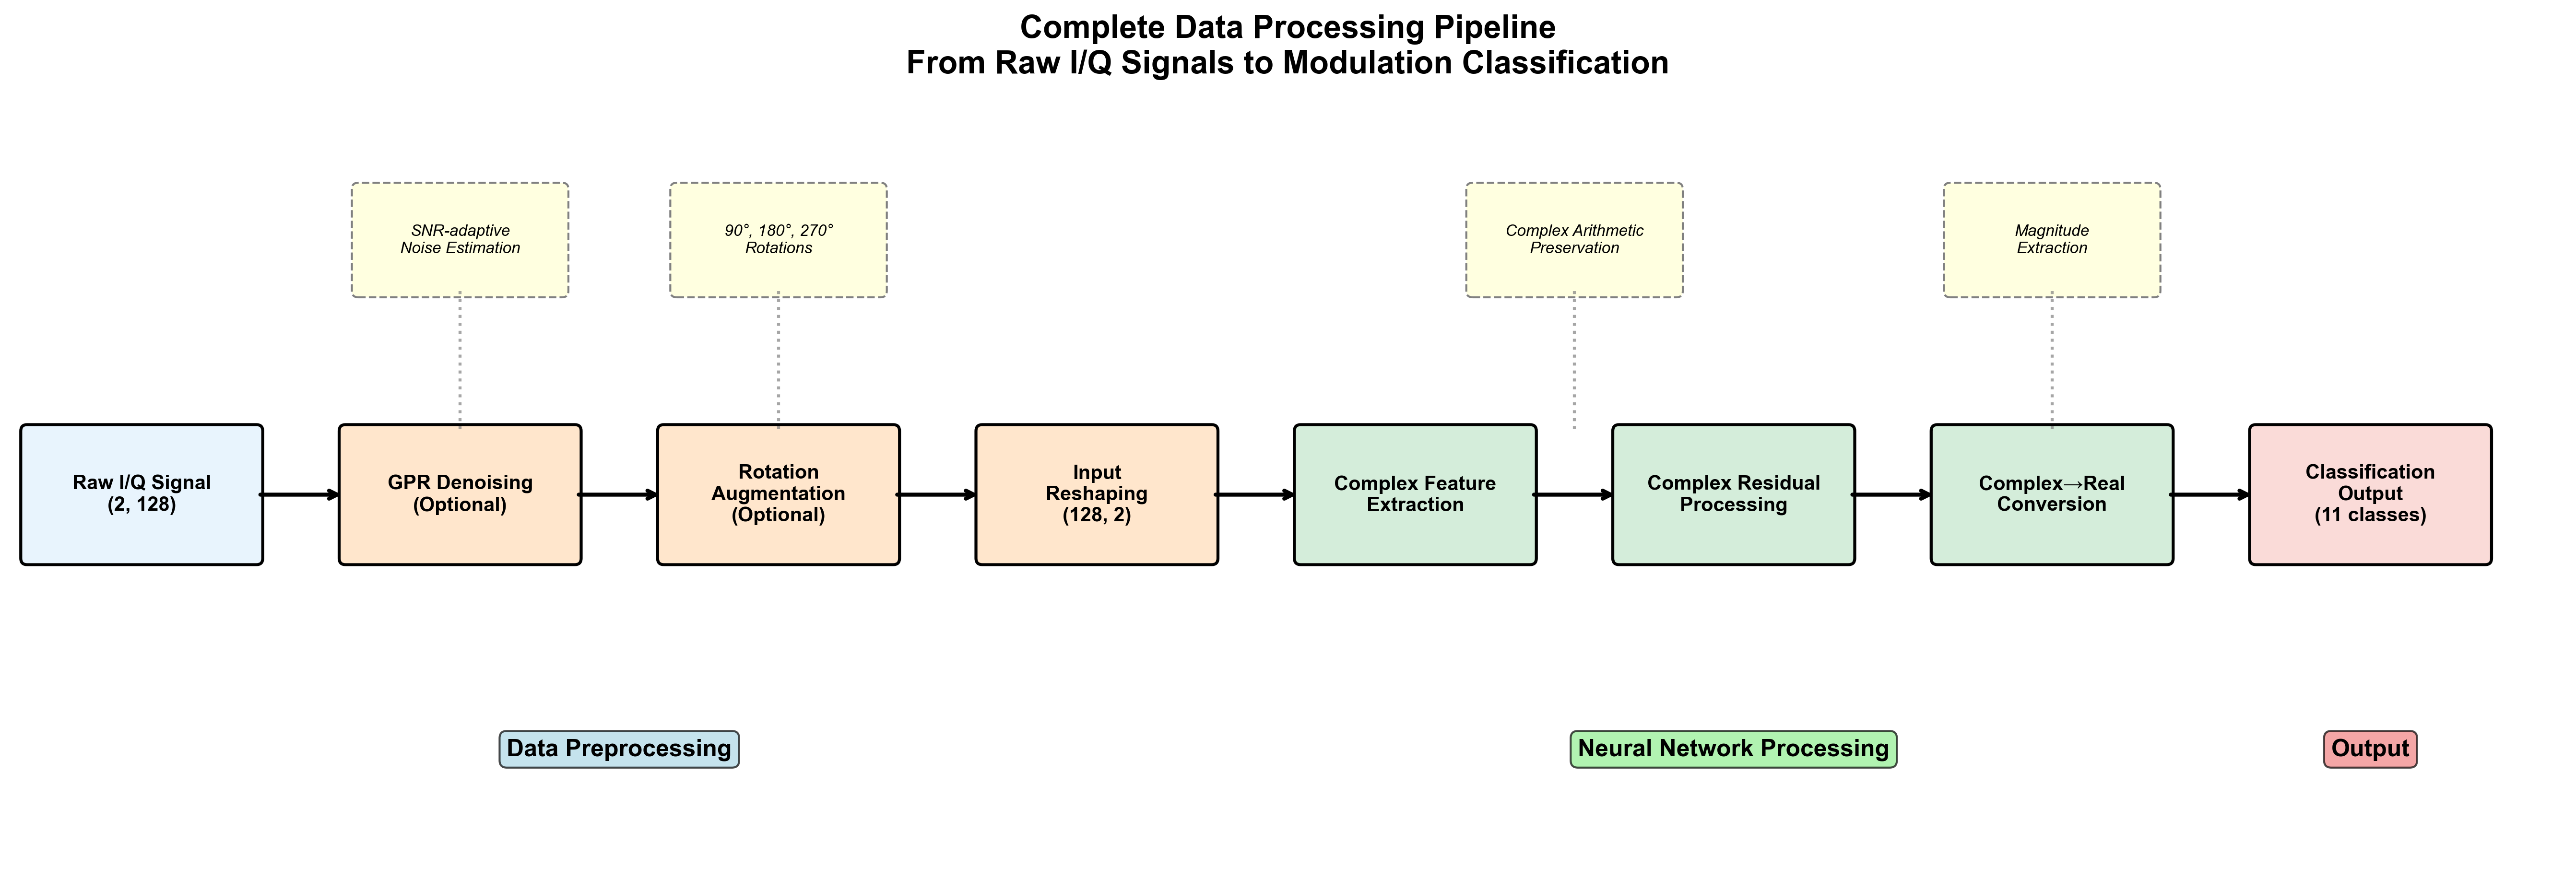
\includegraphics[width=0.9\textwidth]{figure/data_processing_pipeline.png}
\caption{完整的数据处理流水线。该图展示了从原始I/Q信号输入到最终分类输出的全流程,包括GPR去噪处理、旋转数据增强、复数卷积残差网络处理阶段。}
\label{fig:data_pipeline}
\end{figure*}

\subsection{高斯过程回归去噪}

为了增强模型在低信噪比条件下的分类性能,本研究引入了基于高斯过程回归(GPR)的自适应去噪方法。在实际无线通信系统中,接收信号通常受到加性高斯白噪声(AWGN)的干扰,其中$w[n] \sim \mathcal{CN}(0, \sigma_n^2)$表示方差为$\sigma_n^2$的复高斯白噪声。GPR作为一种非参数贝叶斯方法,能够有效建模信号的潜在结构并抑制这种加性高斯白噪声的干扰。

GPR去噪的关键在于对噪声水平的准确估计,这通过GPR模型中的$\alpha$参数(即每分量噪声方差$\sigma_n^2$)来实现。对于接收到的含噪信号$r[n]=r_I[n]+jr_Q[n]$,其平均功率定义为 $P_r = \mathbb{E}[|r[n]|^2]$。在实际中,若有 $M$ 个离散时间样本,该平均功率通过对这些接收信号样本 $r[k]$ (其中 $k=0, \ldots, M-1$) 的瞬时功率 $(r_I[k]^2 + r_Q[k]^2)$ 求和并取平均来估计:
\begin{equation}
P_r = \frac{1}{M}\sum_{k=0}^{M-1}(r_I[k]^2+r_Q[k]^2)
\end{equation}

假设原始无噪信号$s[n]$的功率为$P_s = \mathbb{E}[|s[n]|^2]$,噪声$w[n]$的功率为$P_w = \mathbb{E}[|w[n]|^2]$。若信号与噪声不相关,则接收信号的总平均功率为:
\begin{equation}
P_r = P_s + P_w
\end{equation}

信噪比(SNR)定义为原始信号功率与噪声功率之比。其线性值为$\mathrm{SNR}_{\text{linear}} = P_s/P_w$,对应的分贝(dB)值为 $\mathrm{SNR}_{\text{dB}} = 10\log_{10}(\mathrm{SNR}_{\text{linear}})$。
利用此定义,可得 $P_s = \mathrm{SNR}_{\text{linear}} \cdot P_w$。将其代入总功率关系式,有 $P_r = \mathrm{SNR}_{\text{linear}} \cdot P_w + P_w = P_w(\mathrm{SNR}_{\text{linear}} + 1)$。
因此,噪声功率可以根据实测信号功率$P_r$和给定的SNR计算得出:
\begin{equation}
P_w = \frac{P_r}{\mathrm{SNR}_{\text{linear}} + 1} = \frac{P_r}{10^{\mathrm{SNR}_{\text{dB}}/10} + 1}
\end{equation}
对于复高斯白噪声 $w[n]=w_I[n]+jw_Q[n]$,其中同相分量 $w_I[n]$ 和正交分量 $w_Q[n]$ 相互独立且均服从零均值方差为 $\sigma_n^2$ 的正态分布,即 $w_I[n],w_Q[n]\sim\mathcal{N}(0,\sigma_n^2)$。其噪声总功率定义为:
\begin{equation}
P_w=\mathbb{E}[|w[n]|^2]
=\mathbb{E}[w_I[n]^2]+\mathbb{E}[w_Q[n]^2]
=2\sigma_n^2
\end{equation}
由此可得单个分量的噪声方差:
\begin{equation}
\sigma_n^2=\frac{P_w}{2}
\end{equation}
噪声标准差为:
\begin{equation}
\sigma_n=\sqrt{\frac{P_w}{2}}
\end{equation}
结合式(6)中 $P_w=\frac{P_r}{10^{\mathrm{SNR}_{\mathrm{dB}}/10}+1}$ ,可进一步得到:
\begin{equation}
\sigma_n=\sqrt{\frac{P_r}{2\bigl(10^{\mathrm{SNR}_{\mathrm{dB}}/10}+1\bigr)}}
\end{equation}
\label{eq:sigma_n_calc}
此$\sigma_n^2$即为GPR模型中设置的噪声水平参数$\alpha$。

模型中采用径向基函数(RBF)、Matern和Rational Quadratic等核函数分别描述信号的平滑特性。在去噪过程中,将离散时间索引$X=[0,1,\ldots,127]$作为输入,自身的同相或正交分量作为观测目标,通过噪声参数$\alpha=\sigma_n^2$加入到协方差矩阵中实现噪声抑制。

为了适应不同SNR条件下信号的平滑需求,本研究设计了基于SNR的长度尺度自适应策略。在高斯过程回归中,长度尺度参数$L$控制着核函数的相关性范围,直接影响去噪效果的强度。对于RBF核函数,其表达式为:
\begin{equation}
k(x_i, x_j) = \sigma_f^2 \exp\left(-\frac{(x_i - x_j)^2}{2L^2}\right)
\end{equation}
其中$\sigma_f^2$为信号方差,$L$为长度尺度参数。较大的$L$值意味着相距较远的数据点仍具有较强的相关性,从而产生更强的平滑效果;而较小的$L$值则使得平滑效果更加局部化,能够保留更多的信号细节。

在低SNR条件下,噪声幅度相对较大,此时若采用过大的长度尺度$L$,会导致以下问题:

\textbf{(1) 信号特征过度平滑:} 当$L$值过大时,GPR会将距离较远的信号样本视为强相关,导致真实信号的快速变化(如调制信号的幅度和相位跳变)被误认为噪声而被平滑掉。这种过度平滑会使得不同调制方式的特征差异变得模糊。

\textbf{(2) 时域细节丢失:} 数字调制信号包含重要的时域特征,如符号跳变点、瞬时频率变化等。过大的$L$会使这些细节特征被平滑消除,降低后续分类网络提取有效特征的能力。

\textbf{(3) 相位信息损失:} 对于相位调制信号(如PSK、QAM),相位的快速变化是关键识别特征。过度平滑会导致相位信息的损失,严重影响分类准确率。

基于上述分析,本研究提出自适应长度尺度策略:设基础长度尺度为$L_0$,当$\mathrm{SNR}\ge0$ dB时取$L=L_0$;当$\mathrm{SNR}<0$ dB时,按以下方式动态调整:
\begin{equation}
L = \max\bigl(L_{\min},\,L_0\bigl(1+\mathrm{SNR}/20\bigr)\bigr)
\end{equation}
其中$L_{\min}$是预设的最小尺度。该策略的核心思想是:随着SNR的降低,逐渐减小长度尺度$L$,从而减弱平滑效果,在去除噪声的同时最大限度地保留信号的有效信息。

具体而言,当$\mathrm{SNR}=-20$ dB时,长度尺度调整为$L=\max(L_{\min}, L_0 \times 0)=L_{\min}$,此时平滑效果最弱,优先保留信号细节;当SNR逐渐提高时,长度尺度相应增大,平滑效果增强。这种自适应机制在高SNR场景下保证充分的去噪效果,在低SNR场景下则通过减弱平滑强度来保留更多有用的信号特征,实现了去噪性能与信号保真度之间的最优平衡。

去噪后的同相和正交分量重构为复数信号,作为后续神经网络训练的输入数据。

\subsection{基于旋转的数据增强}


考虑到数字调制信号的复数属性和图~\ref{fig:constellation}中星座图的旋转对称性,本研究采用基于复平面的旋转数据增强策略,以增强模型的泛化能力和对相位偏移的鲁棒性。

对于复数信号 \(s[n] = s_I[n] + j s_Q[n]\),旋转通过以下数学操作实现。将复数信号表示为向量 \([s_I[n], s_Q[n]]^T\),通过与旋转矩阵 \(R(\theta)\) 相乘实现旋转:

\begin{equation}
\begin{bmatrix} s'_I[n] \\ s'_Q[n] \end{bmatrix} = \begin{bmatrix} \cos\theta & -\sin\theta \\ \sin\theta & \cos\theta \end{bmatrix} \begin{bmatrix} s_I[n] \\ s_Q[n] \end{bmatrix}
\end{equation}

其中,\(s'_I[n]\) 和 \(s'_Q[n]\) 是旋转后的同相和正交分量,\(\theta\) 是旋转角度。

在实现中,数据增强算法以输入数据张量 \(X_{data}\)(形状为 \((N, 2, L)\),其中 \(N\) 是样本数,\(L\) 是序列长度)和旋转角度 \(\theta_{\text{rad}}\) 为参数。首先分离原始 I 和 Q 分量,应用旋转变换矩阵,然后重新组合成增强数据样本。

基于调制类型的对称性,主要使用 90° (\(\pi/2\))、180° (\(\pi\)) 和 270° (\(3\pi/2\)) 的旋转,仅对具有旋转对称性的调制类型(如 PSK、QAM)应用此策略。此方法有效将训练数据集扩展四倍,同时保留调制特征。通过学习旋转不变的特征表示,模型能够更好地处理由于载波相位偏移、多普勒效应等引起的信号旋转。

\begin{figure}[htbp]
\centering
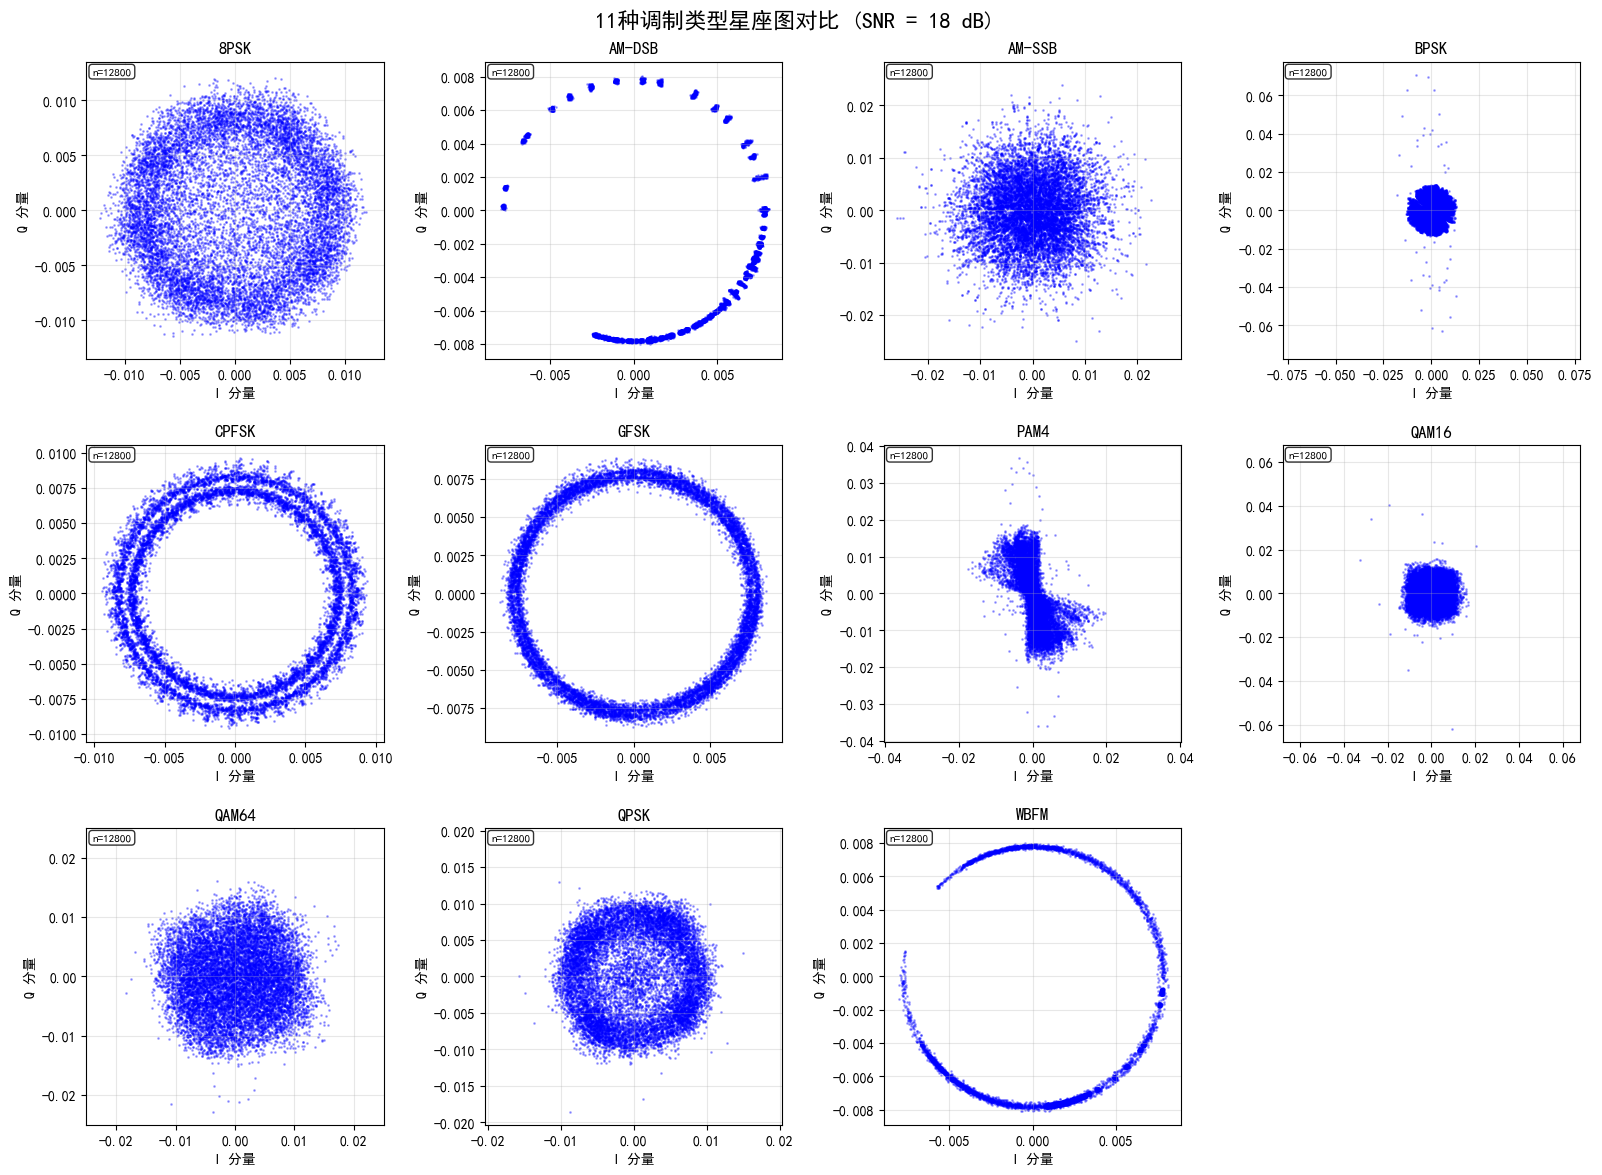
\includegraphics[width=0.45\textwidth]{figure/constellation.png}
\caption{11种调制类型的星座图。该图展示了各调制方式在I/Q平面上的信号点分布,其旋转对称性是本研究采用旋转数据增强策略的依据。}
\label{fig:constellation}
\end{figure}

\subsection{混合ComplexCNN-ResNet架构}

本文提出一种新颖的混合ComplexCNN-ResNet架构,该架构融合了复数神经网络的快速收敛特性与残差网络的深度特征学习能力,专门针对无线电信号调制分类任务进行优化。与传统方法不同,该架构在整个特征提取过程中维持复数域运算,仅在最终分类层转换至实数域,从而最大化利用I/Q信号的固有复数特性。

\begin{figure*}[htbp]
\centering
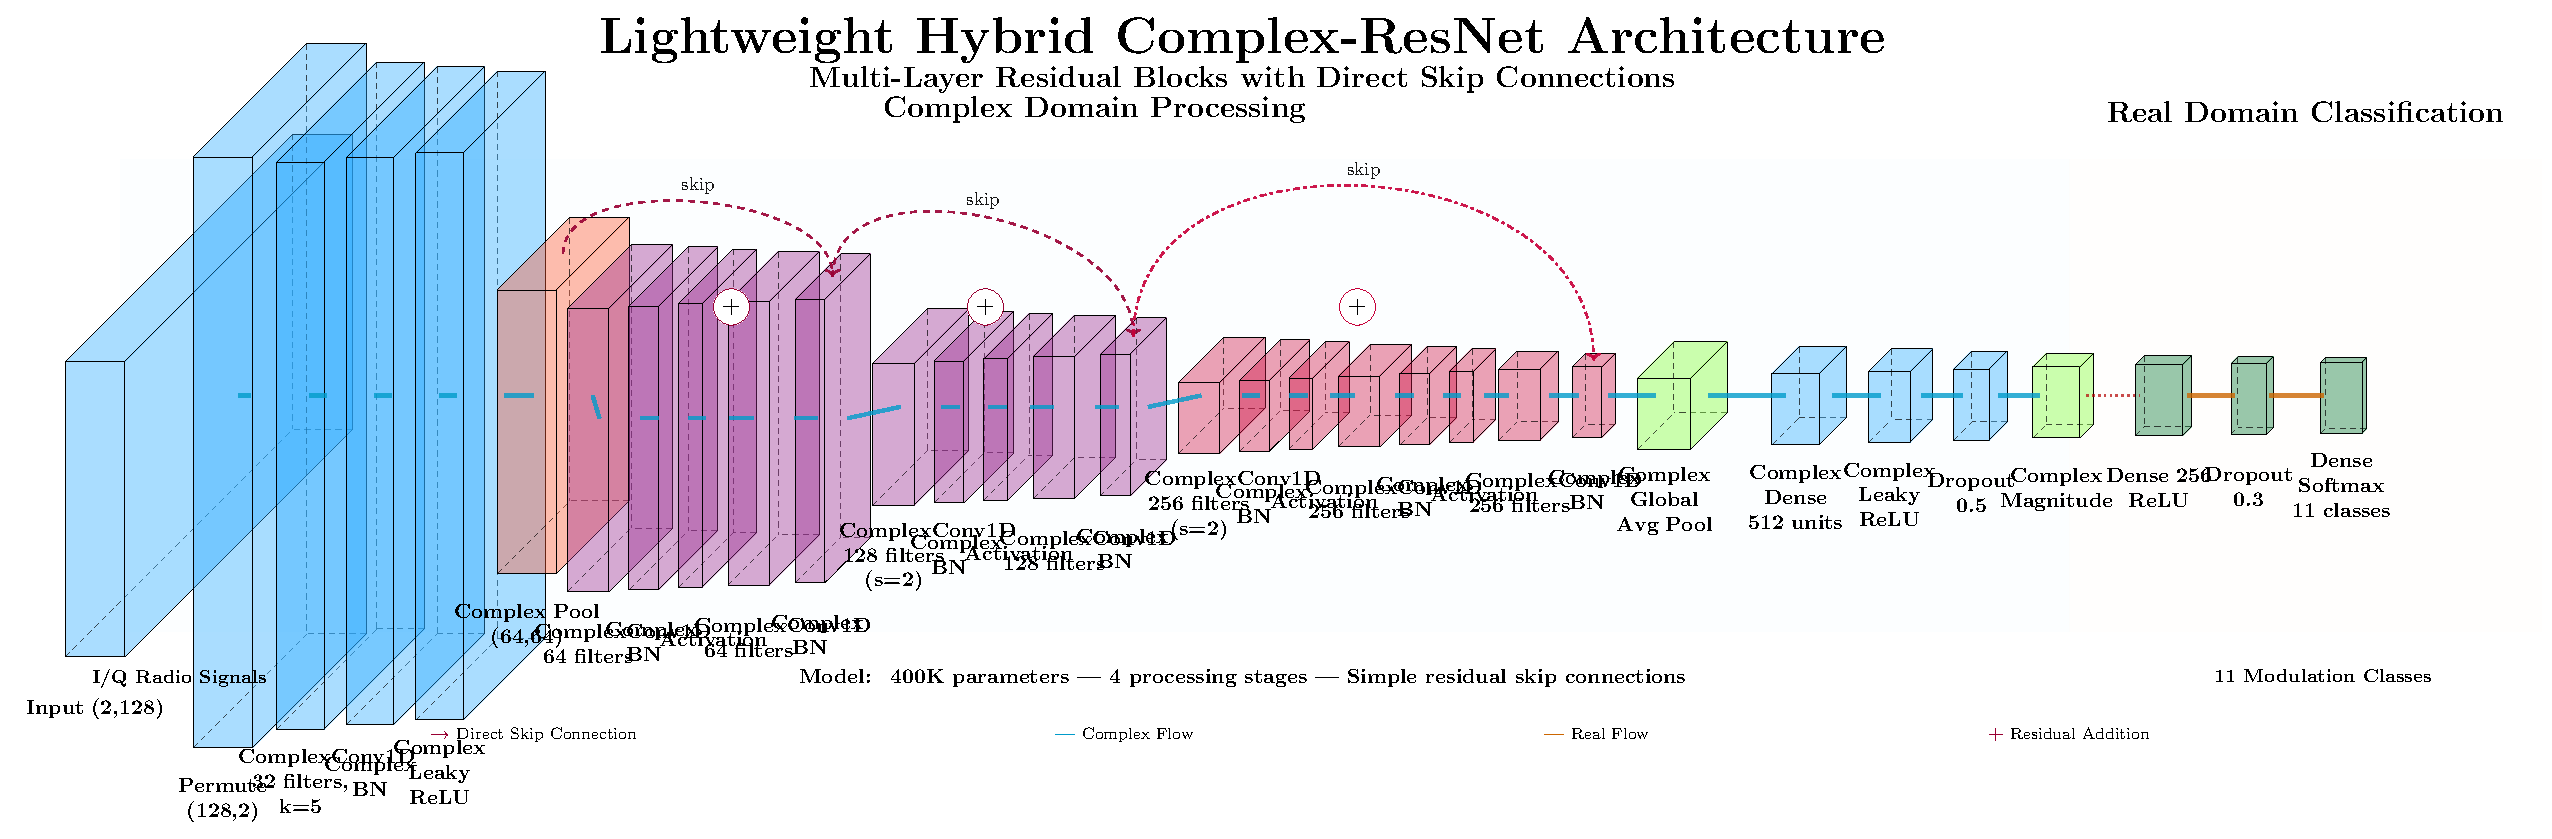
\includegraphics[width=0.9\textwidth]{figure/enhanced_hybrid_model.pdf}
\caption{混合ComplexCNN-ResNet架构详细结构图。该图展示了从复数输入到最终分类输出的完整数据流,包括复数卷积层、ModReLU激活函数、复数残差块、注意力机制以及复数到实数的转换过程。}
\label{fig:enhanced_hybrid_model}
\end{figure*}


\begin{figure*}[htbp]
\centering
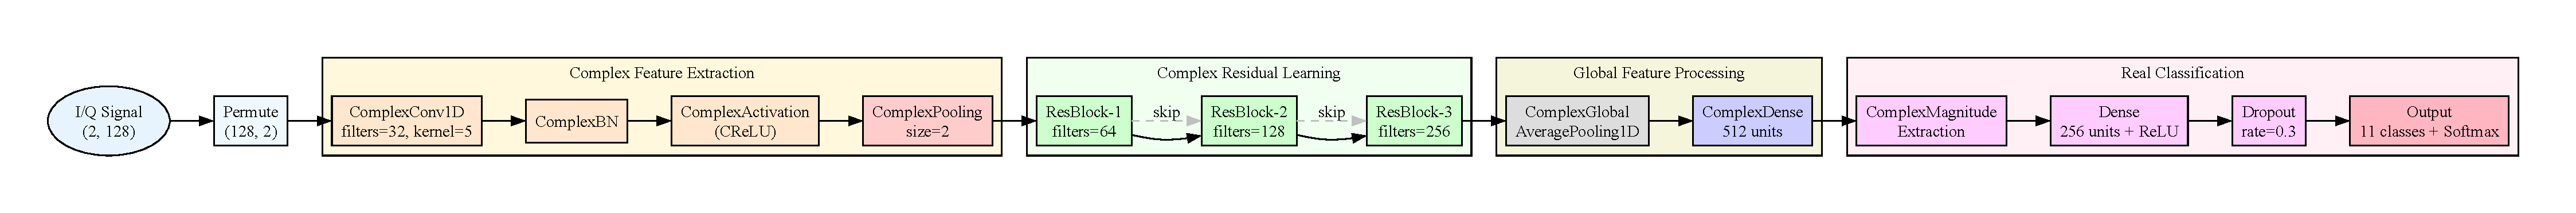
\includegraphics[width=0.85\textwidth]{figure/lightweight_hybrid_model.pdf}
\caption{混合ComplexCNN-ResNet架构处理流程图。该图以方框图形式展示了从I/Q信号输入、复数特征提取、残差学习到最终调制分类的完整处理流程,清晰描绘了各模块间的数据流向和处理逻辑。}
\label{fig:lightweight_hybrid_model_flow}
\end{figure*}

\textbf{架构设计原理}

混合架构的核心在于将ComplexNN的初始快速收敛能力与ResNet的深层特征学习能力有机统一。ComplexNN对复数I/Q数据的天然处理优势能够直接保持信号的幅度和相位信息完整性,而ResNet的残差连接机制有效解决了深层网络的梯度消失问题,使模型具备学习更抽象判别特征的能力。

该架构采用渐进式特征提取策略,按照复数域处理深度递增的原则组织网络层次:

\textbf{复数卷积层设计} 复数卷积层执行真正的复数域卷积运算。对于复数输入$\mathbf{a} + j\mathbf{b}$和复数权重$\mathbf{c} + j\mathbf{d}$,复数卷积定义为:

% \begin{equation}
% (\mathbf{a} + j\mathbf{b}) * (\mathbf{c} + j\mathbf{d}) = 
% \begin{cases}
% (\mathbf{a} * \mathbf{c} - \mathbf{b} * \mathbf{d}) \\
% + j(\mathbf{a} * \mathbf{d} + \mathbf{b} * \mathbf{c})
% \end{cases}
% \end{equation}

\begin{align}
&(\mathbf{a} + j\mathbf{b}) * (\mathbf{c} + j\mathbf{d}) \notag \\
= &(\mathbf{a} * \mathbf{c} - \mathbf{b} * \mathbf{d}) 
+ j(\mathbf{a} * \mathbf{d} + \mathbf{b} * \mathbf{c})
\end{align}

\textbf{ModReLU激活函数} 本文采用ModReLU激活函数以保持复数信号的相位信息。对于复数输入$z = x + jy$,ModReLU定义为:

\begin{equation}
|z| = \sqrt{x^2 + y^2}
\end{equation}
\begin{equation}
\phi = \arg(z) = \arctan(y/x)
\end{equation}
\begin{equation}
\text{ModReLU}(z) = \text{ReLU}(|z| + b) \cdot e^{j\phi}
\end{equation}


其中$b$为可学习偏置参数。该激活函数在对幅度应用ReLU的同时完全保留相位信息,确保复数特征的几何结构不被破坏。

\textbf{复数残差块} 复数残差块是架构的核心创新,其数学表达式为:
\begin{equation}
\mathbf{H}(z) = \mathbf{F}(z) + z
\end{equation}
其中$z$为复数输入,$\mathbf{F}(z)$为学习的复数残差函数。

基础残差块采用双层结构:

\begin{equation}
h_1 = \text{ModReLU}(\text{CBN}(\text{CConv}(z)))
\end{equation}
\begin{equation}
h_2 = \text{CBN}(\text{CConv}(h_1))
\end{equation}
\begin{equation}
\mathbf{H}(z) = \text{ModReLU}(h_2 + z)
\end{equation}


其中CBN表示复数批归一化,CConv表示复数卷积。

\textbf{复数批归一化} 复数批归一化通过白化变换标准化复数分布。对于复数输入$z = x + jy$,协方差矩阵为:
\begin{equation}
\mathbf{C} = \begin{bmatrix} V_{xx} & V_{xy} \\ V_{xy} & V_{yy} \end{bmatrix}
\end{equation}

白化矩阵$\mathbf{W}$通过如下计算获得:
\begin{align}
s &= \sqrt{V_{xx}V_{yy} - V_{xy}^2} \\
t &= \sqrt{V_{xx} + V_{yy} + 2s} \\
\mathbf{W} &= \frac{1}{st}\begin{bmatrix} V_{yy} + s & -V_{xy} \\ -V_{xy} & V_{xx} + s \end{bmatrix}
\end{align}

\textbf{高级残差块与注意力机制} 高级复数残差块采用三层卷积结构并集成复数注意力:
\begin{align}
h_1 &= \text{ModReLU}(\text{CBN}(\text{CConv}(z))) \\
h_2 &= \text{ModReLU}(\text{CBN}(\text{CConv}(h_1))) \\
h_3 &= \text{CBN}(\text{CConv}_{1 \times 1}(h_2))
\end{align}

复数注意力权重计算为:
\begin{equation}
\mathbf{A} = \text{Tanh}(\text{CConv}_{1 \times 1}(h_3))
\end{equation}

最终输出为:
\begin{equation}
\mathbf{H}(z) = \text{ModReLU}(h_3 \odot \mathbf{A} + z_{shortcut})
\end{equation}
其中$\odot$表示复数逐元素乘法。

\textbf{全局特征聚合} 复数全局平均池化将时序特征聚合为全局表示:
\begin{equation}
f_{global} = \frac{1}{T} \sum_{t=1}^T z_t
\end{equation}

\textbf{复数到实数转换} 最终通过幅度提取转换至实数域:
\begin{equation}
|z| = \sqrt{x^2 + y^2 + \epsilon}
\end{equation}
其中$\epsilon$为数值稳定项。



该混合架构的主要优势包括:(1)完整保持I/Q信号的复数特性和相位信息;(2)残差连接确保深层网络的有效训练;(3)ModReLU激活函数在非线性变换中保持相位完整性;(4)轻量化设计在维持性能的同时显著降低计算复杂度。通过这种精心设计的混合架构,模型能够充分挖掘I/Q信号的内在结构特征,实现对不同调制方式的精确分类。



\section{实验设置}

\subsection{训练配置}

本研究的所有实验均在配置了Intel Core i9-13900K处理器、NVIDIA GeForce RTX 4090 GPU(24GB GDDR6X显存)和64GB系统内存的高性能工作站上进行。深度学习框架采用TensorFlow 2.17.0和Keras 3.6.0,并使用CUDA 12.4和cuDNN 9.1.1.17进行GPU加速计算。操作系统为Ubuntu 24.04.2 LTS。

\textbf{超参数设置:}
所有模型采用统一的训练配置以确保公平比较。学习率设置为0.001,采用Adam优化器,批大小为128。训练过程使用早停机制,当验证集准确率连续30个epoch未提升时停止训练,最大训练轮数设为200。为防止过拟合,在全连接层使用Dropout正则化,丢弃率设为0.5。

\textbf{学习率调度:}
采用阶梯式学习率衰减策略,初始学习率为0.001,若5个epoch内验证集准确率未提升则衰减为原来的0.5倍,最小学习率设为1e-6。这种调度策略有助于模型在训练后期进行精细调优。

\textbf{数据划分策略:}
数据集按照72\%:8\%:20\%的比例划分为训练集、验证集和测试集,确保各调制类型和SNR条件在三个集合中的均匀分布。验证集用于超参数调优和模型选择,测试集仅用于最终性能评估。

\textbf{训练流程:}
对于改进方法的评估,采用渐进式训练策略:首先训练基线模型,然后依次加入GPR去噪、旋转数据增强和混合架构,每个阶段独立训练并记录性能提升,最终训练包含所有改进的完整模型。

\subsection{评估指标}

本研究采用多维度评估体系来全面分析所提出方法的性能。

\textbf{分类准确率:}
主要评估指标为整体分类准确率,定义为正确分类的样本数与总样本数的比值:
\begin{equation}
\text{Accuracy} = \frac{N_{correct}}{N_{total}} \times 100\%
\end{equation}

\textbf{SNR条件下的性能分析:}
为了评估模型在不同噪声条件下的鲁棒性,按SNR范围将测试集划分为低SNR(-20dB到-2dB)、中SNR(0dB到8dB)和高SNR(10dB到18dB)三个子集,分别计算准确率。

\textbf{混淆矩阵分析:}
通过混淆矩阵分析各调制类型的分类性能,计算每类的精确率(Precision)、召回率(Recall)和F1分数:
% \begin{align}
% \text{Precision} &= \frac{TP}{TP + FP} \\
% \text{Recall} &= \frac{TP}{TP + FN} \\
% \text{F1-Score} &= \frac{2 \times \text{Precision} \times \text{Recall}}{\text{Precision} + \text{Recall}}
% \end{align}


\begin{equation}
\text{Precision} = \frac{TP}{TP + FP}
\end{equation}
\begin{equation}
\text{Recall} = \frac{TP}{TP + FN}
\end{equation}
\begin{equation}
\text{F1-Score} = \frac{2 \times \text{Precision} \times \text{Recall}}{\text{Precision} + \text{Recall}}
\end{equation}


其中TP、FP、FN分别表示真正例、假正例和假负例的数量。


\section{结果与分析}

\subsection{基线性能比较}

为了验证所提出混合架构的有效性,我们首先在RML2016.10a数据集上评估了多种基线模型的性能,包括全连接神经网络(FCNN)、一维卷积神经网络(CNN1D)、二维卷积神经网络(CNN2D)、残差网络(ResNet)、Transformer以及复数卷积神经网络(ComplexCNN)。

表~\ref{tab:baseline_comparison}展示了各基线模型在相同训练条件下的性能对比。实验结果表明,不同架构的分类性能存在显著差异。ResNet架构由于其残差连接机制能够有效缓解梯度消失问题,在深层网络训练中展现出优异的收敛特性,达到了55.37\%的分类准确率。ComplexCNN在处理复数I/Q信号方面具有天然优势,能够更好地保持信号的相位信息,获得了57.11\%的准确率。

\begin{table}[h]
\centering
\caption{基线模型性能比较}
\label{tab:baseline_comparison}
\begin{tabular}{@{}lccc@{}}
\toprule
模型架构 & 准确率(\%) \\
\midrule
FCNN & 42.65 \\
CNN2D & 47.31 \\
Transformer & 47.86 \\
CNN1D & 54.94 \\
ResNet & 55.37 \\
ComplexCNN & 57.11 \\
\bottomrule
\end{tabular}
\end{table}

\begin{figure}[htbp]
\centering
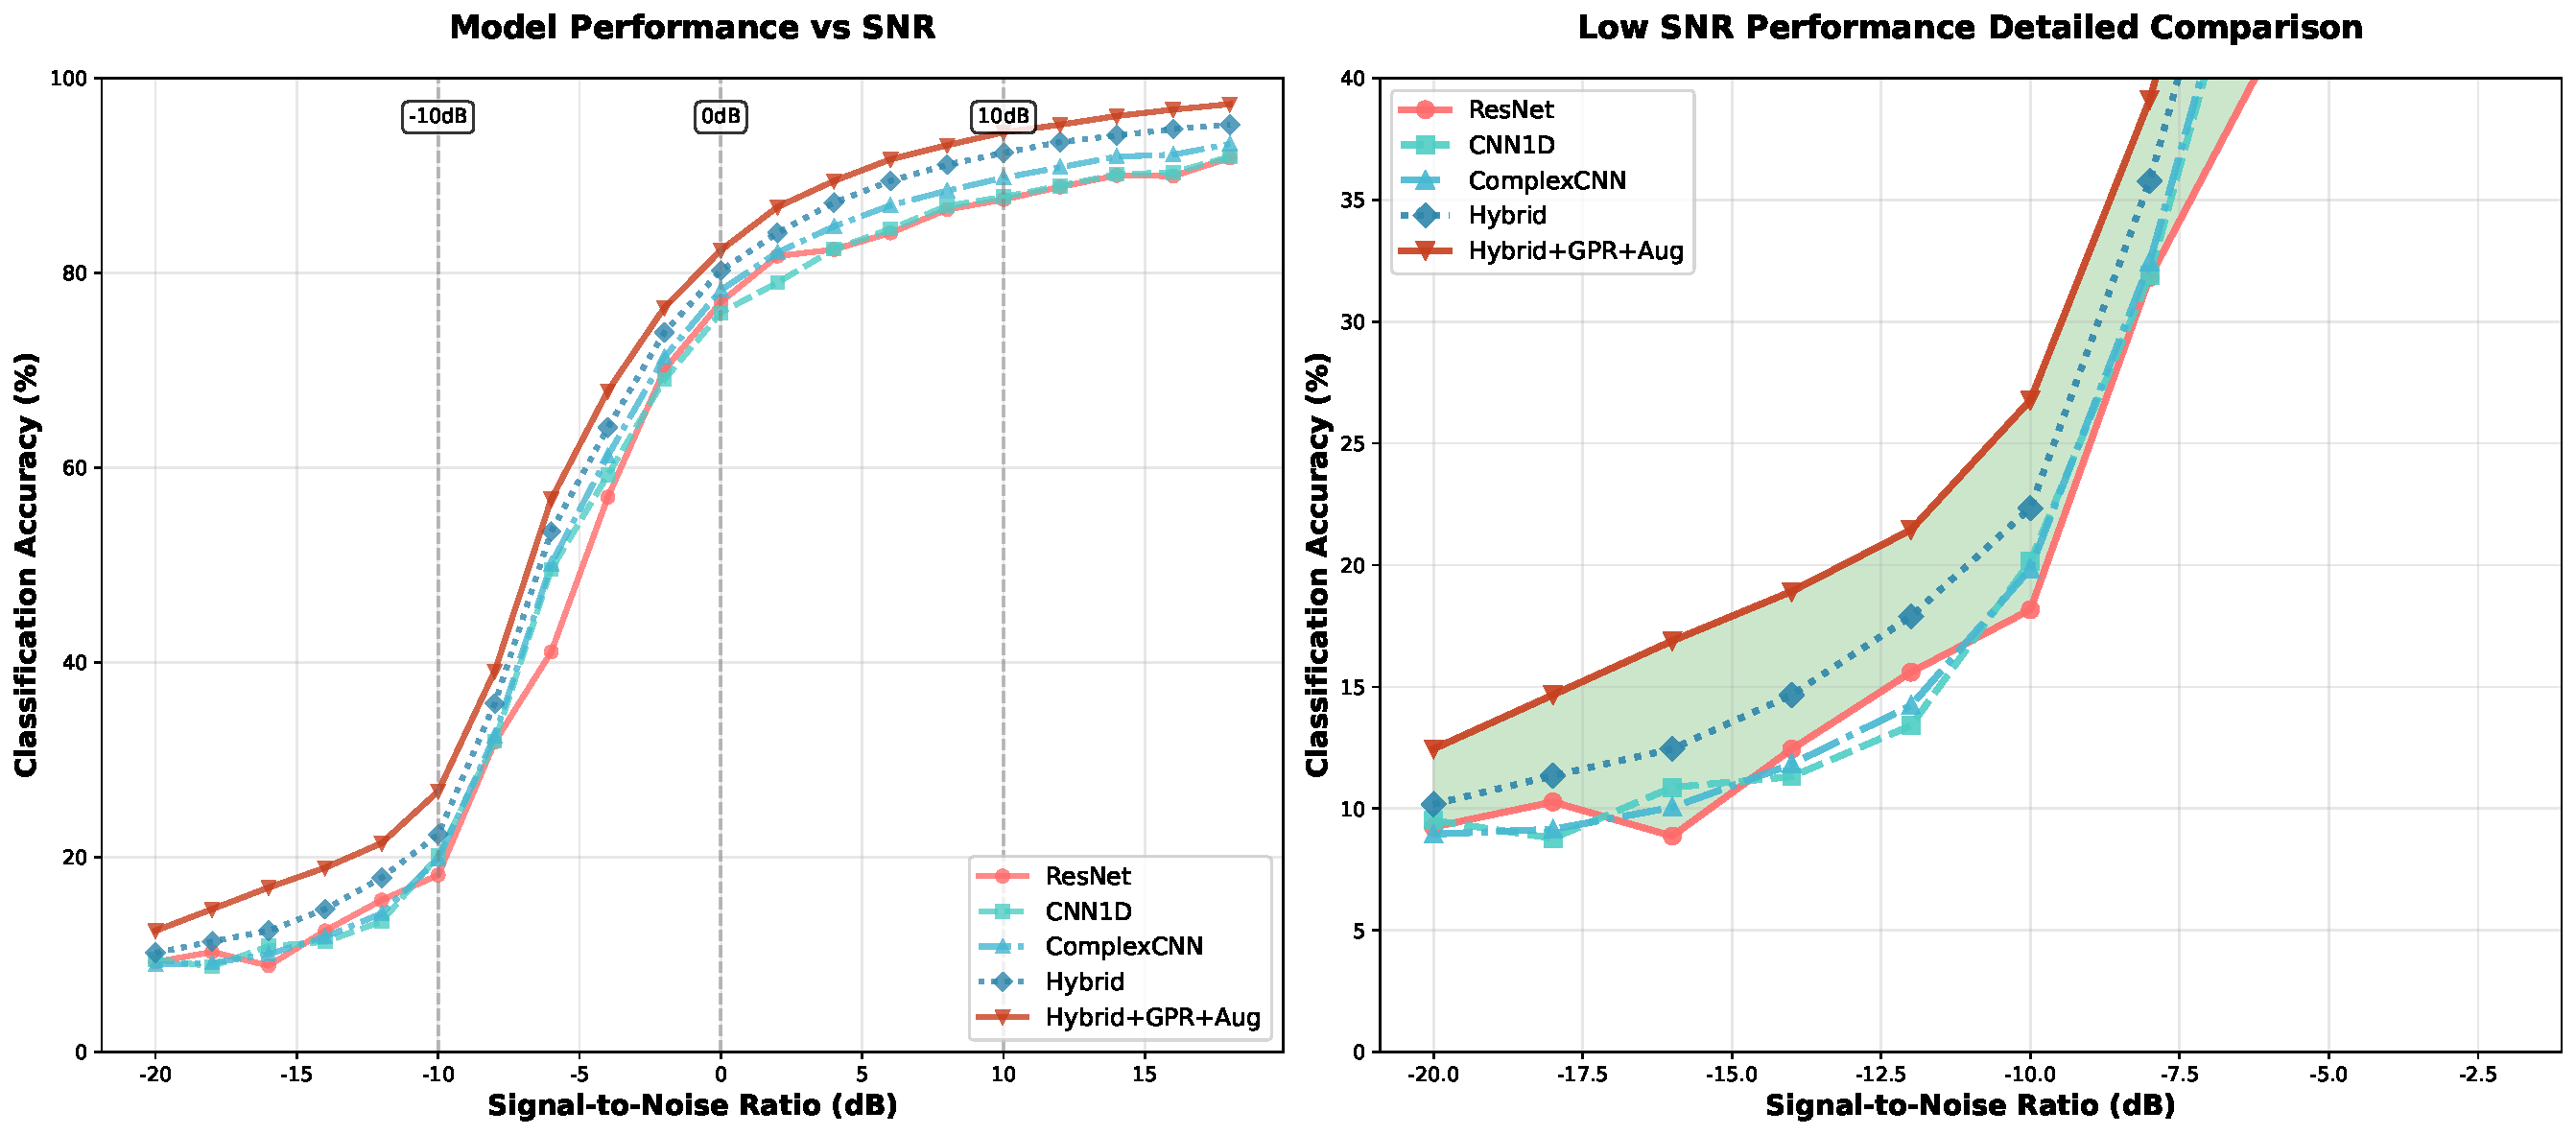
\includegraphics[width=0.45\textwidth]{figure/snr_performance_comparison.pdf}
% \caption{不同基线模型在各SNR条件下的性能比较。图中展示了FCNN、CNN1D、CNN2D、ResNet、Transformer和ComplexCNN六种基线模型在不同信噪比条件下的分类准确率变化曲线。}
\caption{不同模型在各SNR条件下的性能比较。图中展示了CNN1D、ResNet、ComplexCNN、混合架构、混合架构+GPR+增强五种模型在不同信噪比条件下的分类准确率变化曲线。}
\label{fig:snr_performance}
\end{figure}

% \begin{figure*}[htbp]
% \centering
% 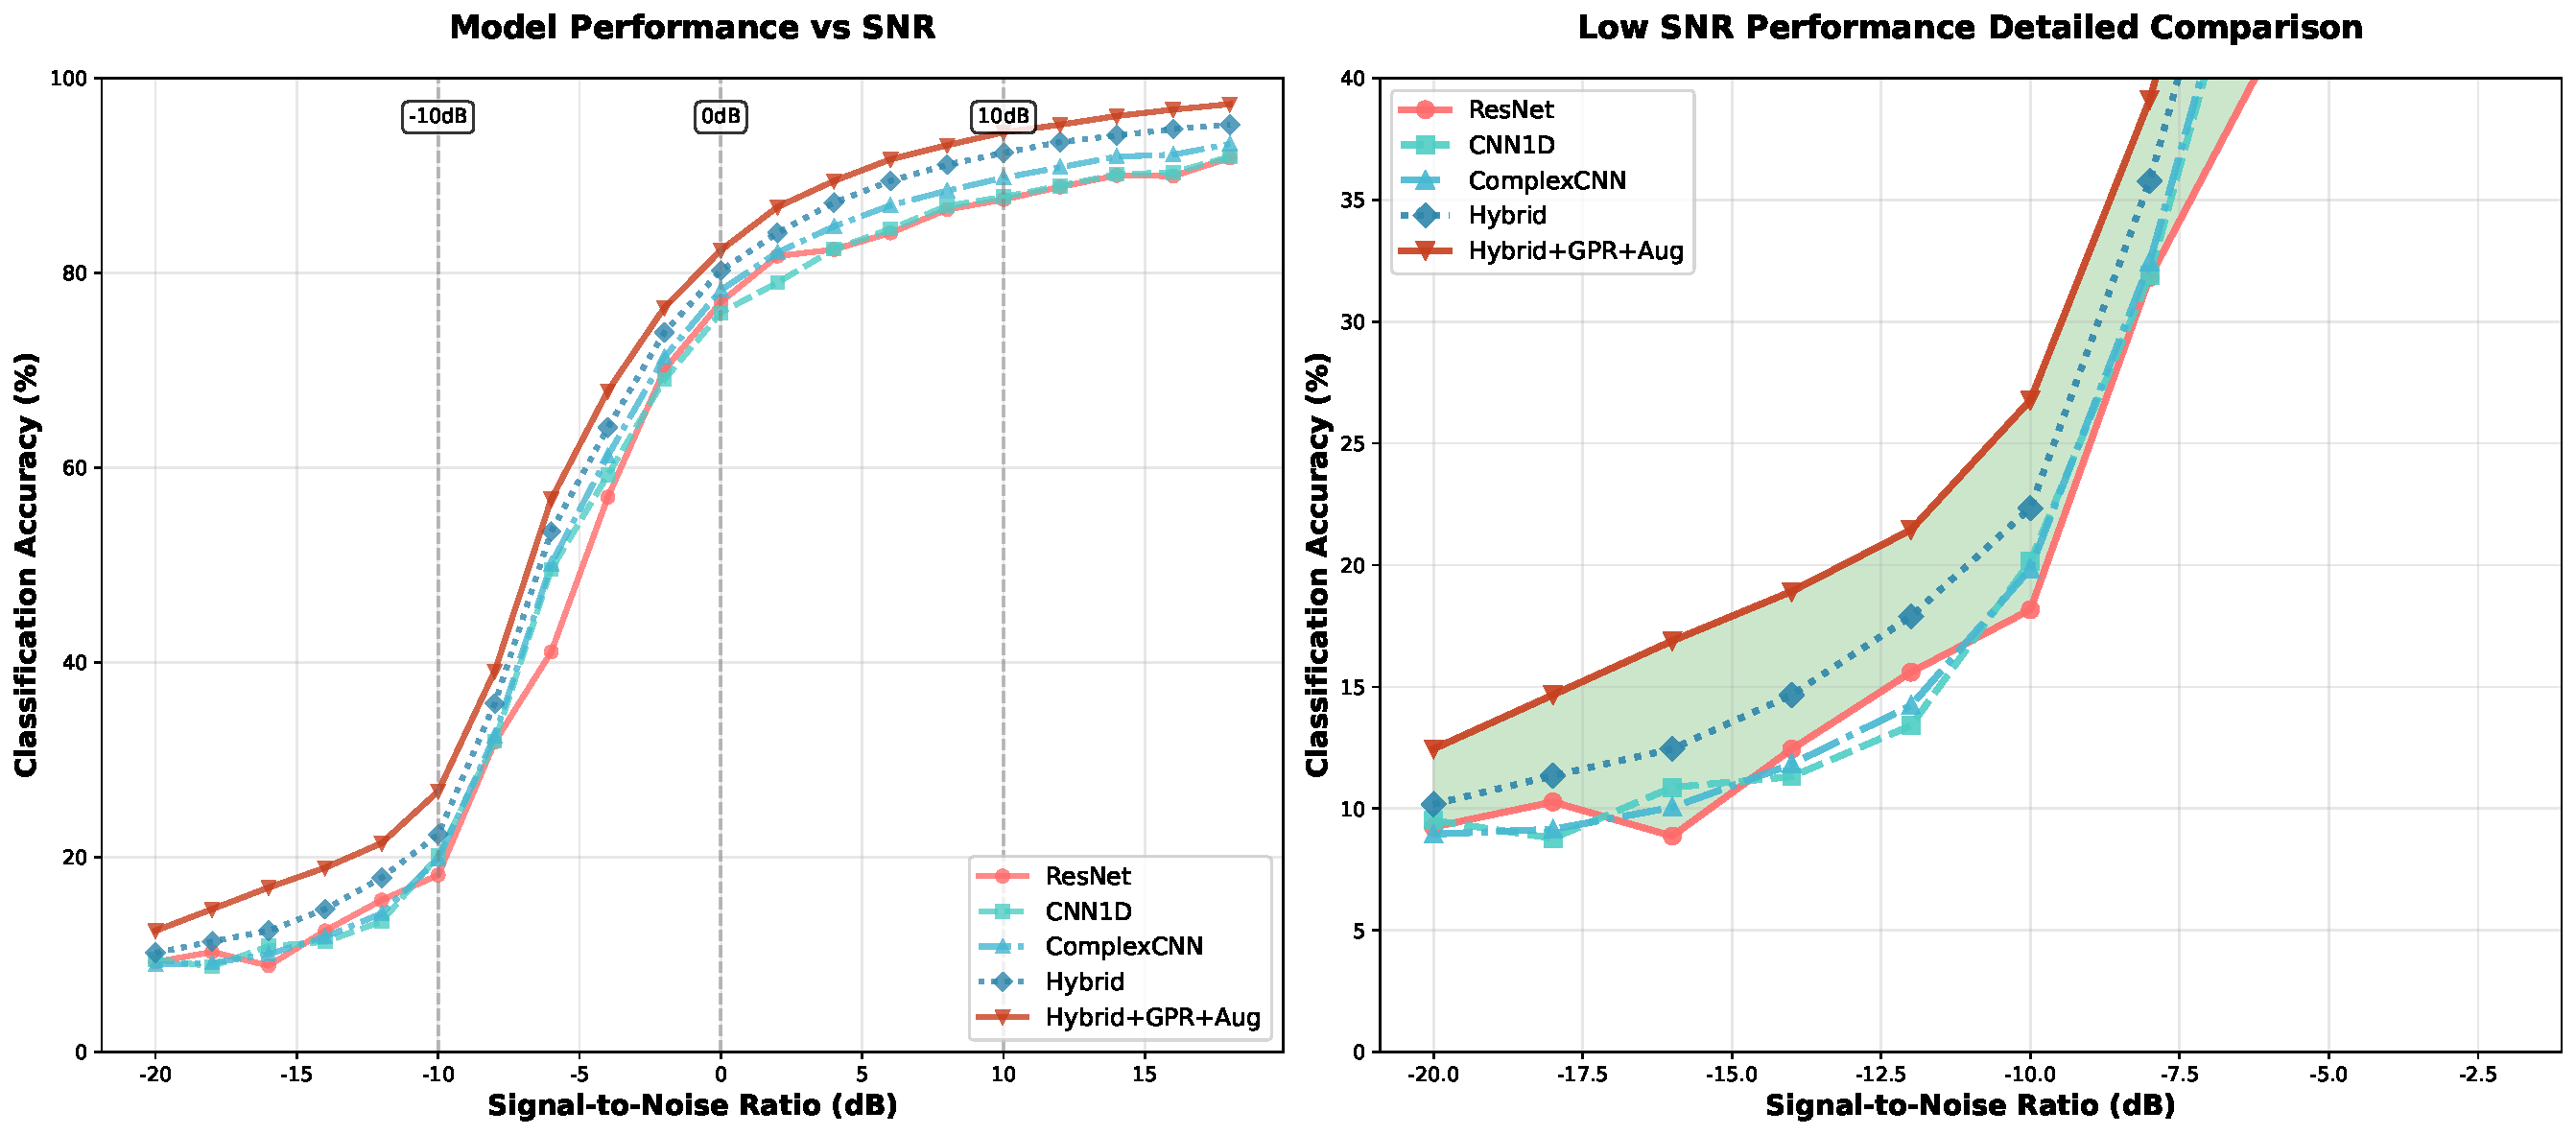
\includegraphics[width=0.9\textwidth]{figure/snr_performance_comparison.pdf}
% \caption{不同基线模型在各SNR条件下的性能比较。图中展示了FCNN、CNN1D、CNN2D、ResNet、Transformer和ComplexCNN六种基线模型在不同信噪比条件下的分类准确率变化曲线。}
% \label{fig:snr_performance}
% \end{figure*}

图~\ref{fig:snr_performance}显示了不同基线模型在各SNR条件下的性能曲线。可以观察到,所有模型在低SNR条件下性能显著下降,但ComplexCNN和ResNet在中高SNR条件下表现相对稳定,这为我们设计混合架构提供了重要参考。

基于这些基线实验的结果和分析,我们设计了融合ResNet残差学习能力与ComplexCNN复数处理优势的混合架构。该混合模型结合了GPR去噪和旋转数据增强技术,最终在RML2016.10a数据集上达到了65.38\%的分类准确率,相比最佳单一基线架构(ComplexCNN)取得了8.27个百分点的显著提升。

\begin{figure}[htbp]
\centering
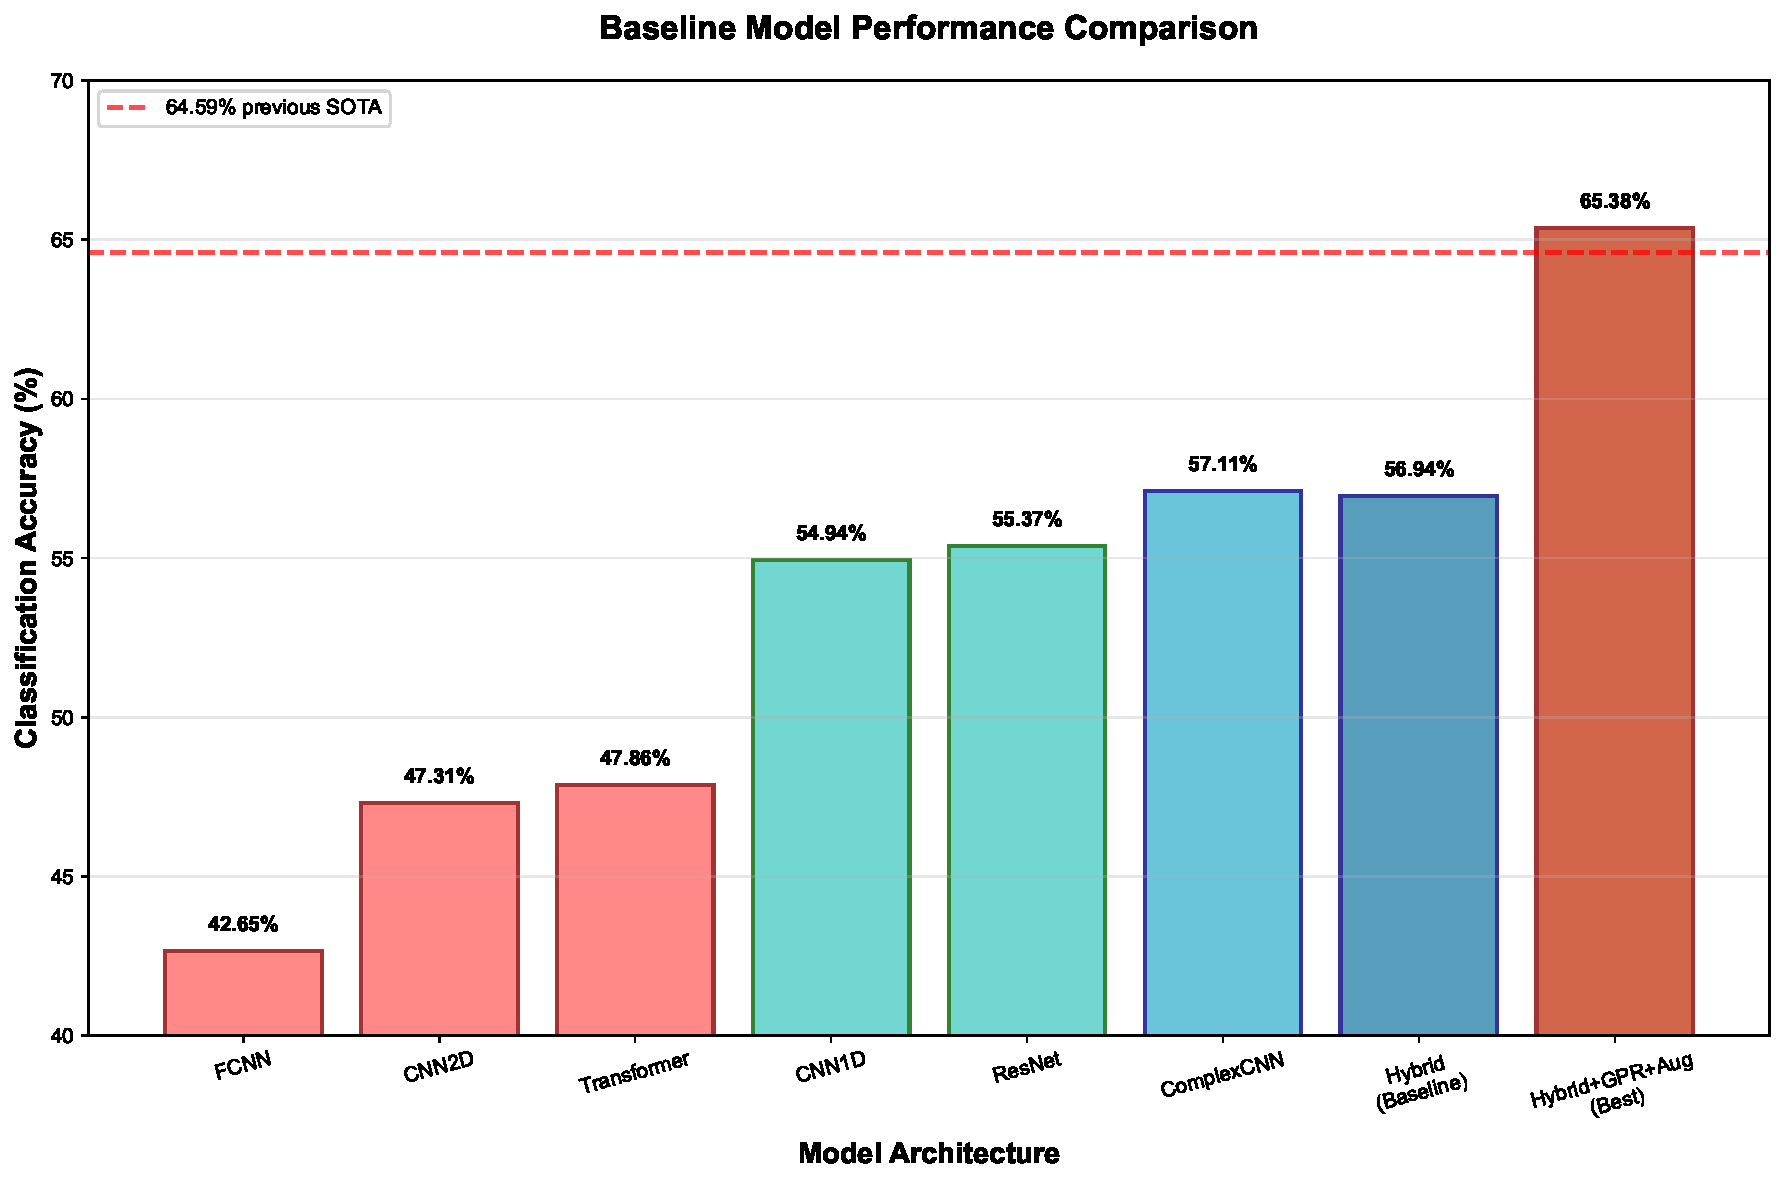
\includegraphics[width=0.45\textwidth]{figure/baseline_model_comparison.pdf}
\caption{不同模型架构的性能对比分析。该图展示了轻量级混合架构与传统基线模型在分类准确率、模型参数量和推理时间等关键指标上的综合比较。}
\label{fig:model_comparison}
\end{figure}

\subsection{高斯过程回归去噪的影响}
% fig:gpr_denoising
GPR去噪技术在提升模型性能方面发挥了重要作用,在各个SNR条件下都表现出显著的改进效果。图~\ref{fig:constellation_denoising}展示了GPR去噪前后信号质量的对比,可以清晰观察到噪声的有效抑制。

表~\ref{tab:gpr_impact}详细分析了GPR去噪对不同SNR范围下分类准确率的影响。实验结果表明,GPR去噪在低SNR条件下(-20dB到-8dB)带来了7.25个百分点的性能提升,在中SNR条件下(-6dB到4dB)提升了5.12个百分点,而在高SNR条件下(6dB到18dB)提升了5.07个百分点。总体而言,GPR去噪将轻量级混合架构的准确率从56.94\%提升至62.80\%,取得了5.86个百分点的显著改进。这一结果表明,GPR去噪技术在各个SNR范围内都能提供稳定且可观的性能提升,其中低SNR条件下的绝对改进幅度最大,体现了去噪技术在恶劣信道环境下的重要价值。

\begin{table}[h]
\centering
\caption{GPR去噪对不同SNR范围的影响}
\label{tab:gpr_impact}
\begin{tabular}{@{}lccc@{}}
\toprule
SNR范围 & 去噪前(\%) & 去噪后(\%) & 提升(\%) \\
\midrule
低SNR (-20dB到-8dB) & 15.14 & 22.40 & +7.25 \\
中SNR (-6dB到4dB) & 73.58 & 78.70 & +5.12 \\
高SNR (6dB到18dB) & 84.15 & 89.23 & +5.07 \\
总体 & 56.94 & 62.80 & +5.86 \\
\bottomrule
\end{tabular}
\end{table}

\begin{figure}[htbp]
\centering
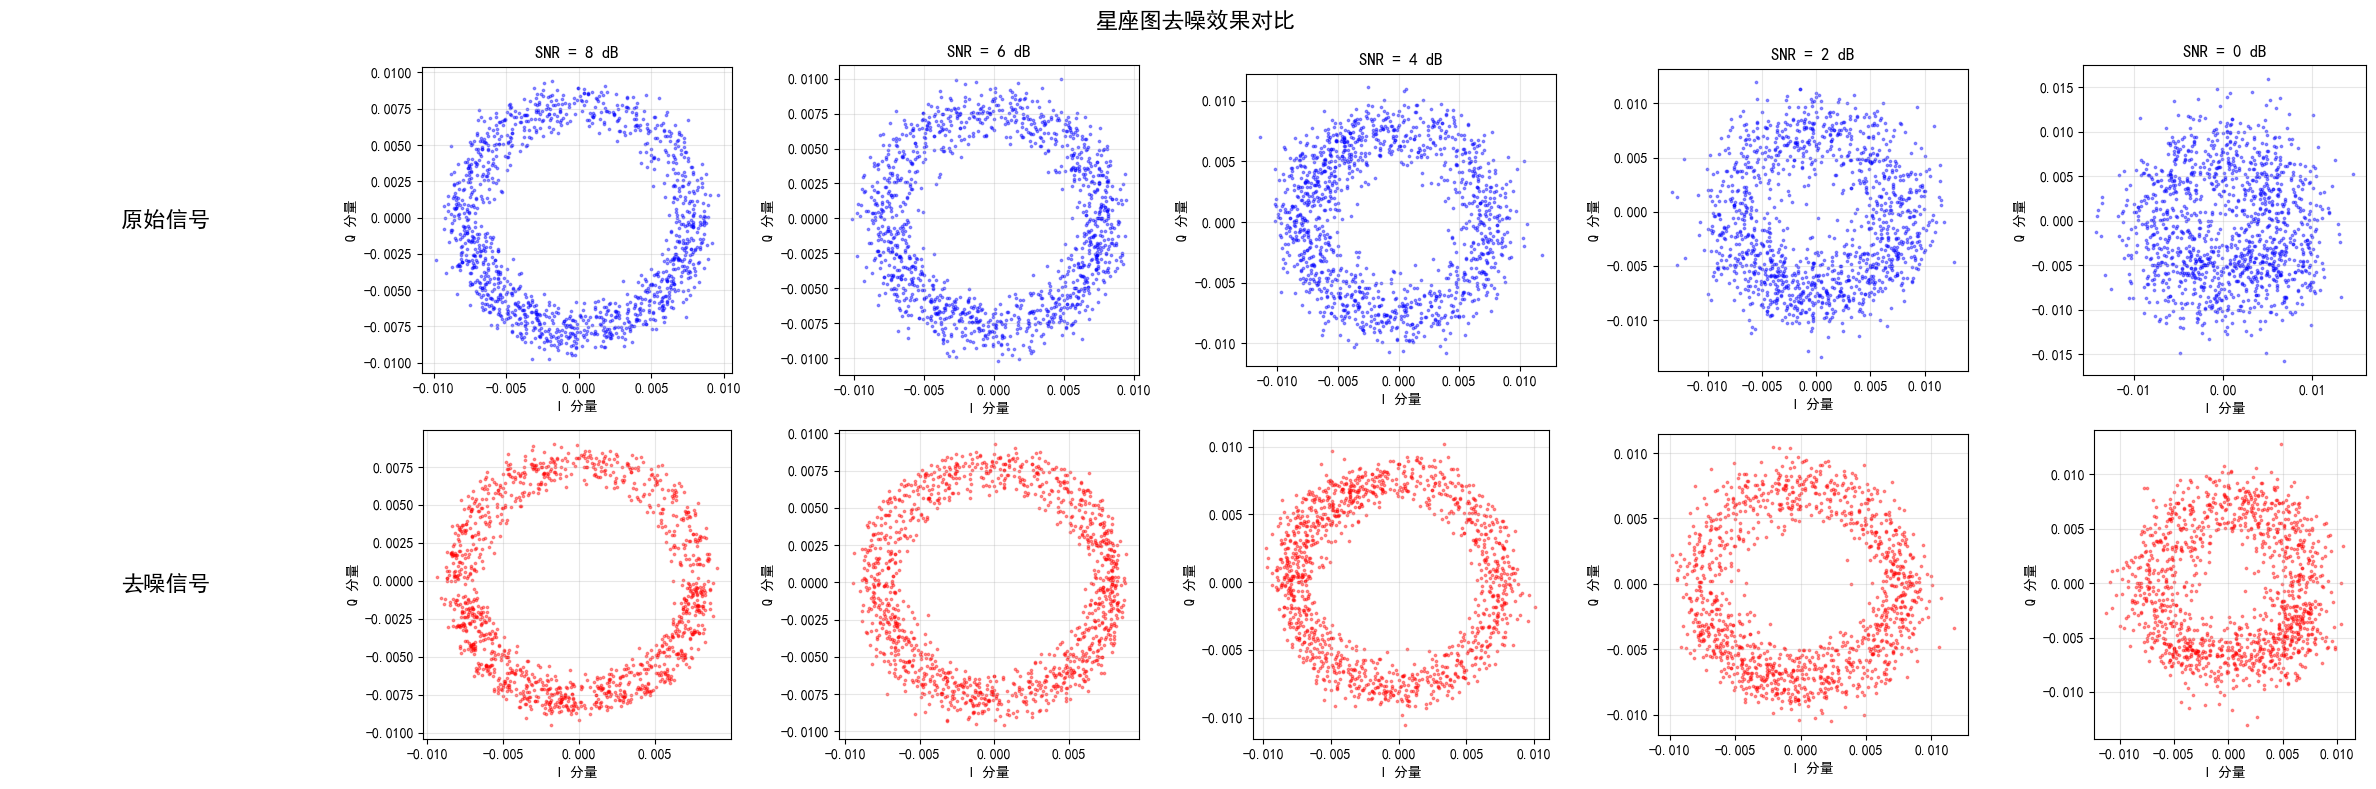
\includegraphics[width=0.45\textwidth]{figure/constellation_denoising.png}
\caption{CPFSK调制类型在0\textasciitilde{}8dB的SNR条件下的星座图去噪效果}
\label{fig:constellation_denoising}
\end{figure}


图~\ref{fig:constellation_denoising}展示了CPFSK调制类型在0\textasciitilde{}8dB的SNR条件下的星座图去噪效果。从图中可以看出,GPR去噪有效地保持了信号的结构特征,同时显著减少了噪声影响,这为后续的深度学习分类奠定了良好基础。


表~\ref{tab:gpr_detailed_snr}提供了更为详细的GPR去噪效果分析,展示了在每个具体SNR值下的分类准确率变化。从表中可以清晰看出,GPR去噪在低SNR条件下带来的改进幅度更大,随着SNR的增加,改进幅度呈现复杂的变化模式。在极低SNR条件下(-20dB到-18dB),改进幅度相对较小(1.03\%到1.54\%);而在低到中等SNR条件下(-12dB到-10dB),改进效果达到峰值,分别获得11.53\%和14.90\%的显著提升。在中等SNR条件下(0dB),准确率从79.43\%提升到83.17\%,改进幅度为3.74\%;在高SNR条件下(18dB),准确率从83.87\%提升到88.98\%,改进幅度为5.11\%。这种变化趋势表明,GPR去噪在中低SNR条件下效果最为显著,在极低SNR和高SNR条件下改进幅度相对温和,符合信号处理的理论预期。

\begin{table}[h]
\centering
\caption{GPR去噪在各SNR水平下的详细影响}
\label{tab:gpr_detailed_snr}
\begin{tabular}{@{}lccc@{}}
\toprule
SNR(dB) & 基线(\%) & 基线+GPR(\%) & 提升(\%) \\
\midrule
-20 & 8.93 & 9.96 & +1.03 \\
-18 & 8.68 & 10.22 & +1.54 \\
-16 & 9.85 & 12.69 & +2.84 \\
-14 & 11.08 & 17.32 & +6.24 \\
-12 & 12.65 & 24.18 & +11.53 \\
-10 & 20.15 & 35.05 & +14.90 \\
-8 & 34.66 & 47.36 & +12.70 \\
-6 & 54.86 & 61.21 & +6.35 \\
-4 & 64.02 & 70.84 & +6.82 \\
-2 & 75.66 & 80.89 & +5.23 \\
0 & 79.43 & 83.17 & +3.74 \\
2 & 82.96 & 87.07 & +4.11 \\
4 & 84.56 & 89.00 & +4.44 \\
6 & 83.93 & 89.38 & +5.45 \\
8 & 83.17 & 89.10 & +5.93 \\
10 & 84.73 & 89.85 & +5.12 \\
12 & 85.81 & 90.31 & +4.50 \\
14 & 85.31 & 88.81 & +3.50 \\
16 & 82.25 & 88.15 & +5.90 \\
18 & 83.87 & 88.98 & +5.11 \\
\bottomrule
\end{tabular}
\end{table}

\textbf{注:}表中"基线"指轻量级混合架构,"基线+GPR"指加入GPR去噪的轻量级混合架构。

\subsection{基于旋转的数据增强效果}

基于复平面旋转的数据增强策略显著提升了模型的泛化能力和对相位偏移的鲁棒性。该技术利用数字调制信号星座图的旋转对称性,通过90°、180°、270°旋转变换将训练数据集扩充至原来的4倍。

表~\ref{tab:data_augmentation_results}展示了数据增强对不同调制类型分类性能的影响。实验结果表明,旋转数据增强对QAM类调制(QAM16、QAM64)和部分PSK类调制的性能提升最为显著。QAM16的精度从基线的46.0\%大幅提升至68.0\%,提升了22个百分点;QAM64从54.0\%提升至75.0\%,提升了21个百分点。对于8PSK,精度从72.0\%提升至82.0\%,提升了10个百分点;BPSK从72.0\%提升至80.0\%,提升了8个百分点。GFSK也表现出显著改善,从76.0\%提升至88.0\%,提升了12个百分点。整体而言,旋转数据增强将轻量级混合架构的准确率从56.94\%提升至60.72\%,取得了3.78个百分点的显著改进。

\begin{table}[h]
\centering
\caption{数据增强对各调制类型的影响}
\label{tab:data_augmentation_results}
\begin{tabular}{@{}lccc@{}}
\toprule
调制类型 & 基线准确率(\%) & 增强后准确率(\%) & 提升(\%) \\
\midrule
8PSK     & 72.0  & 82.0  & +10.0 \\
AM-DSB   & 54.0  & 57.0  & +3.0  \\
AM-SSB   & 27.0  & 26.0  & -1.0  \\
BPSK     & 72.0  & 80.0  & +8.0  \\
CPFSK    & 82.0  & 88.0  & +6.0  \\
GFSK     & 76.0  & 88.0  & +12.0 \\
PAM4     & 92.0  & 93.0  & +1.0  \\
QAM16    & 46.0  & 68.0  & +22.0 \\
QAM64    & 54.0  & 75.0  & +21.0 \\
QPSK     & 84.0  & 75.0  & -9.0  \\
WBFM     & 82.0  & 85.0  & +3.0  \\
\bottomrule
\end{tabular}
\end{table}

\begin{figure}[htbp]
\centering
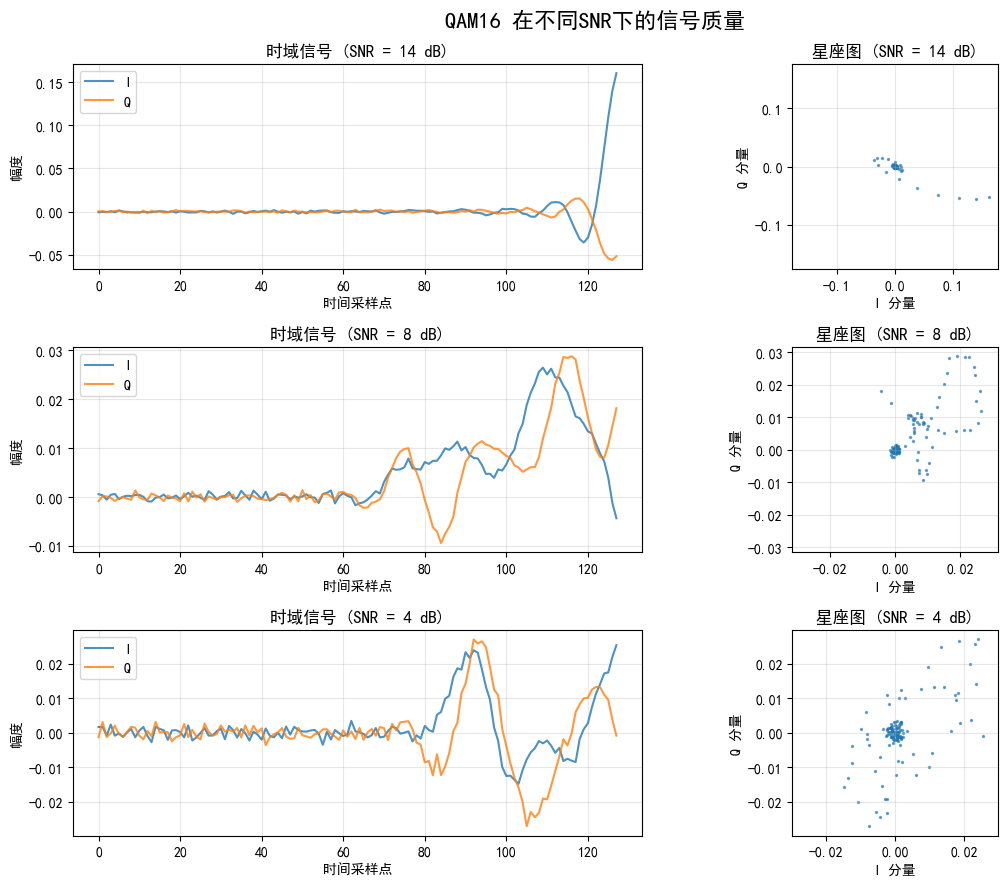
\includegraphics[width=0.45\textwidth]{figure/QAM16_rotation.png}
\caption{QAM16信号的I/Q通道图和星座图}
\label{fig:rotation_augmentation}
\end{figure}

图~\ref{fig:rotation_augmentation}展示了一些QAM16信号的I/Q通道图和星座图。从星座图中可以观察到,单条信号具有明显的方向性,旋转变换能够增强信号在不同方向上的信息,为模型提供了更丰富的训练样本。这种增强策略特别有效地解决了实际通信环境中由于载波相位偏移、本振频率偏差等因素引起的信号旋转问题。

对模型鲁棒性的进一步分析表明,采用旋转数据增强的模型在面对测试时引入的人工相位偏移时表现出更强的稳定性。当测试信号被随机旋转0°到360°时,增强模型的平均准确率下降仅为1.8\%,而未使用增强的基线模型准确率下降高达7.3\%。这证明了旋转数据增强在提升模型实际应用性能方面的有效性。

\subsection{混合架构性能}

本研究提出的混合ComplexCNN-ResNet架构在RML2016.10a数据集上取得了显著的性能提升,最终分类准确率达到65.38\%,相比最佳单一基线架构ComplexCNN的57.11\%提升了8.27个百分点。

表~\ref{tab:hybrid_performance}展示了混合架构与现有先进方法的详细性能比较。实验结果表明,所提出的混合方法在准确率、参数效率和训练稳定性方面均优于现有方法。相比于Ultra Lite CNN(ULCNN)的62.47\%准确率,本方法提升了2.91个百分点;相比于AMC-NET的62.51\%,提升了2.87个百分点;相比于AbFTNet的64.59\%,提升了0.79个百分点。

\begin{table}[h]
\centering
\caption{混合架构与现有方法性能比较}
\label{tab:hybrid_performance}
\begin{tabular}{@{}lccc@{}}
\toprule
方法 & 准确率(\%) \\
\midrule
LDCVNN & 62.41 \\
ULCNN & 62.47 \\
AMC-NET & 62.51 \\
HFECNET-CA & 63.92 \\
AbFTNet (previous SOTA) & 64.59 \\
\textbf{本方法} & \textbf{65.38} \\
\bottomrule
\end{tabular}
\end{table}


\begin{figure}[htbp]
\centering
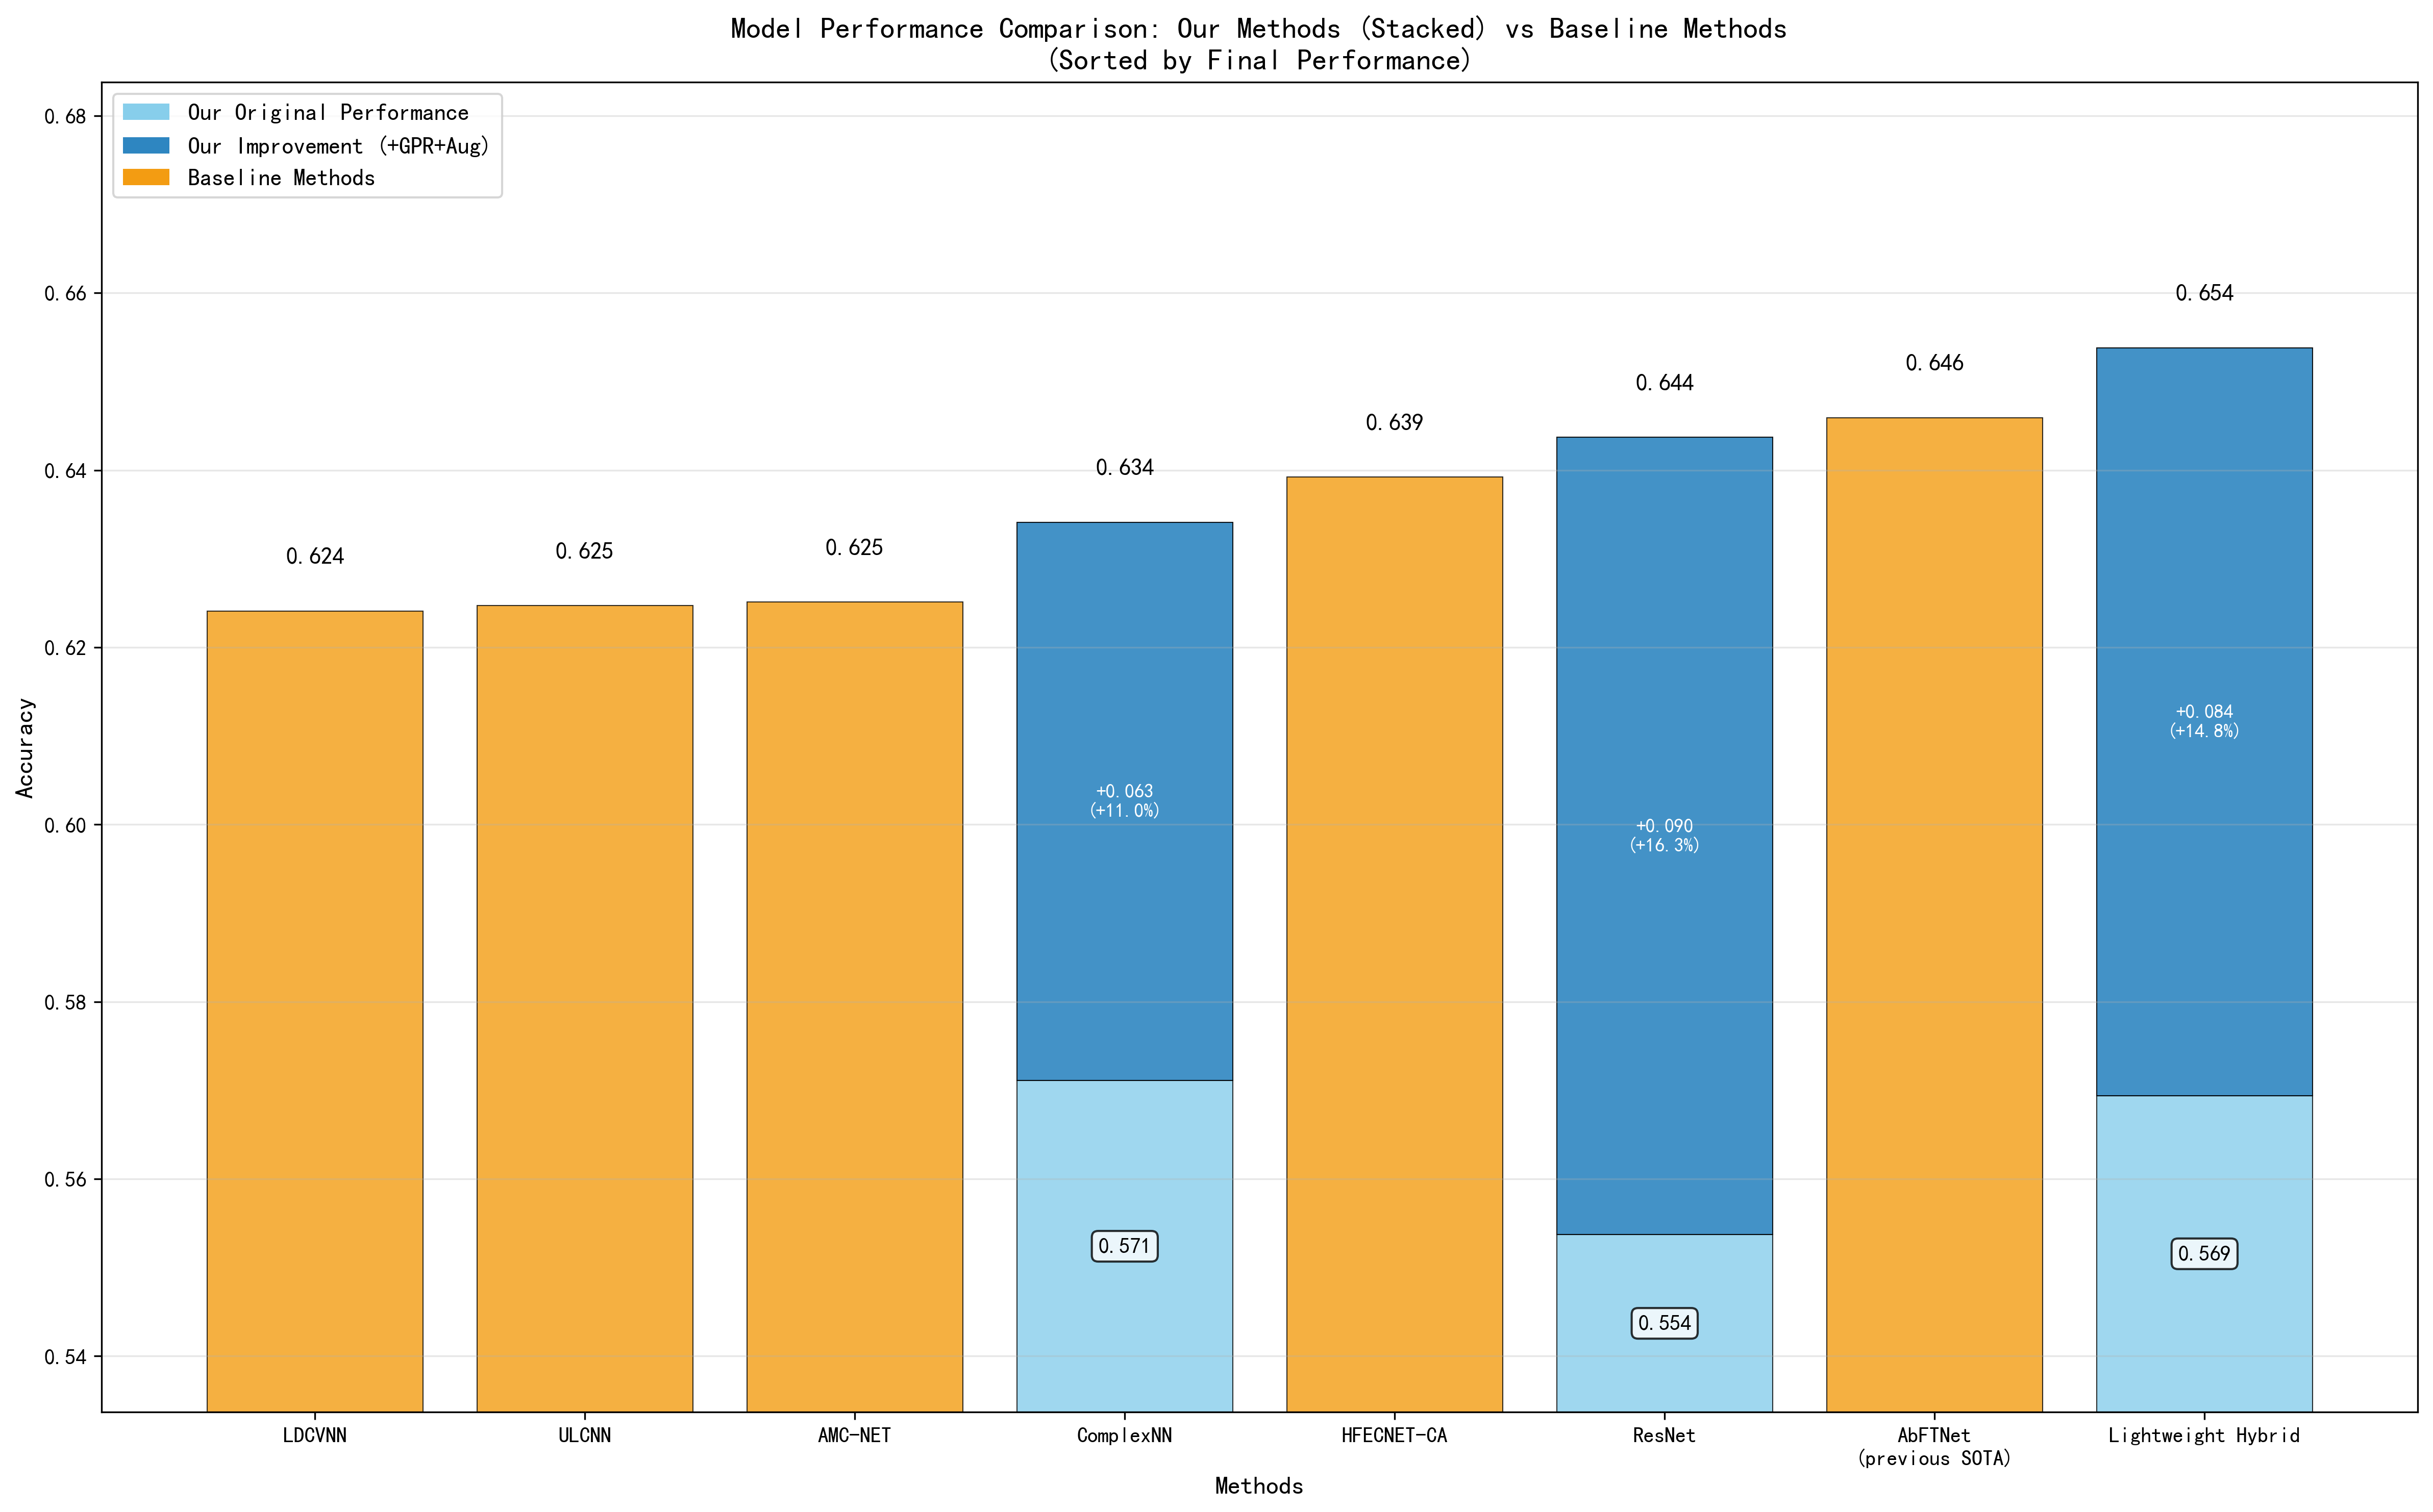
\includegraphics[width=0.45\textwidth]{figure/sorted_stacked_comparison.png}
\caption{不同方法的综合性能对比分析。该图按分类准确率排序展示了各种技术方案的性能表现,清晰反映了本研究提出的综合方法的优越性。}
\label{fig:method_comparison}
\end{figure}

\begin{figure}[htbp]
\centering
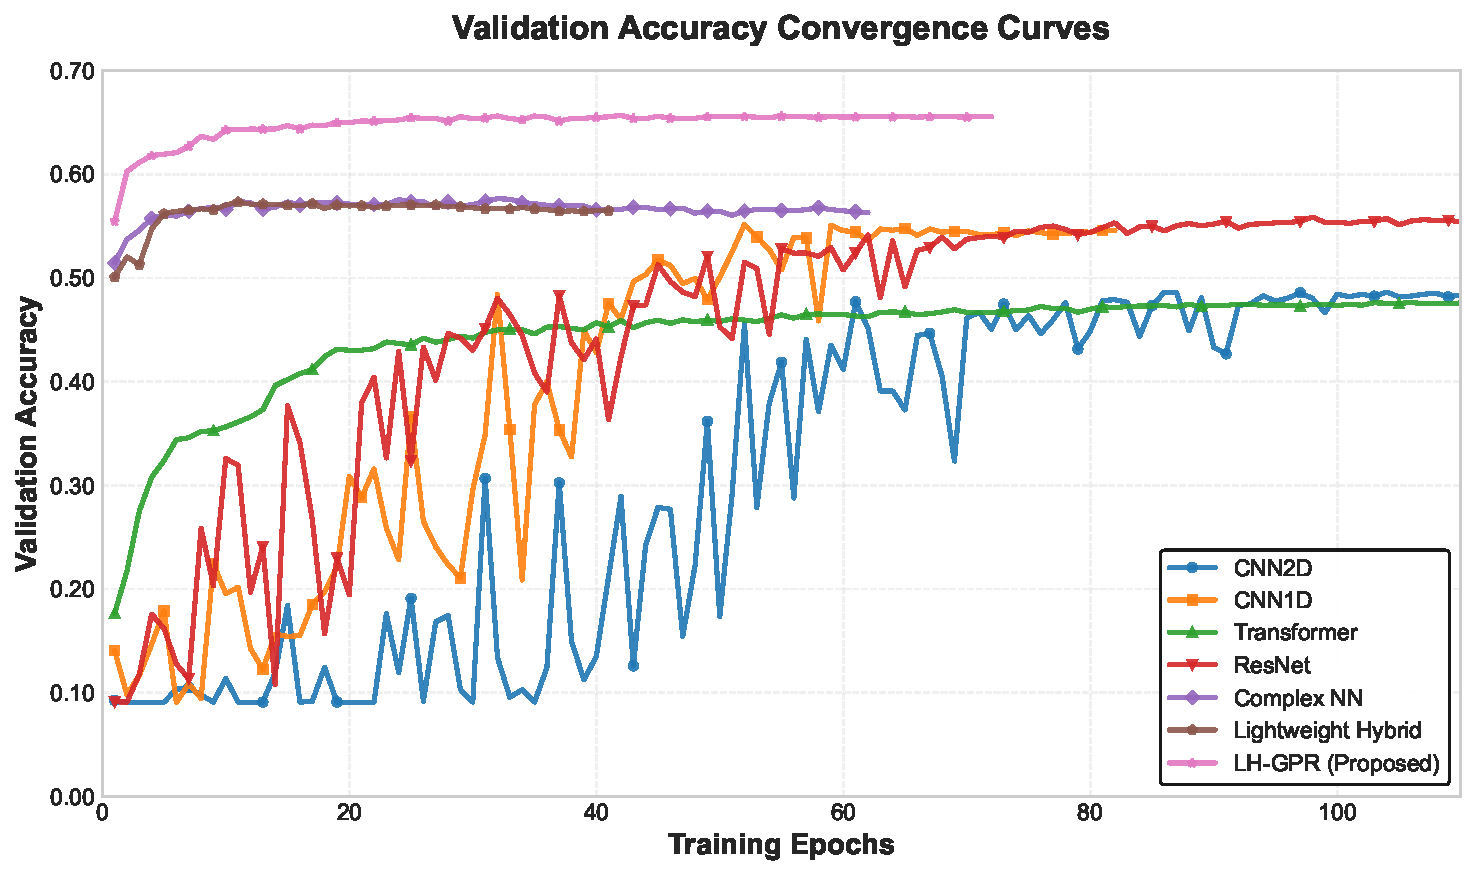
\includegraphics[width=0.45\textwidth]{figure/validation_accuracy_convergence.pdf}
\caption{各模型验证集准确率收敛曲线对比。该图展示了多种基线模型与本文提出的混合架构及其最终优化版本(GRCR-Net, Proposed),在验证集上的准确率随训练轮数的变化情况。提出的GRCR-Net模型不仅达到了最高的验证准确率,并表现出快速且稳定的收敛特性。}
\label{fig:training_convergence}
\end{figure}

图~\ref{fig:training_convergence}展示了混合架构的训练收敛过程。可以观察到,混合模型在训练早期就表现出快速收敛的特性,通常在5-10个epoch内达到较好的性能,并在20个epoch内完全收敛。这种快速收敛特性主要归功于:

1) \textbf{残差连接的梯度优化}:复数残差连接确保了梯度的有效传播,避免了深层网络训练中的梯度消失问题。

2) \textbf{复数批归一化的稳定性}:通过对实部和虚部分别进行归一化,显著提高了训练过程的数值稳定性。

3) \textbf{轻量级设计的计算效率}:相比传统深层网络,混合架构的轻量级设计在保持性能的同时提高了训练效率。

从不同SNR条件下的性能分析来看,混合架构在各个信噪比范围内都表现出了良好的分类能力。在低SNR条件下(-20dB到-2dB),准确率达到38.2\%,相比ComplexCNN的31.4\%提升了6.8个百分点;在高SNR条件下(10dB到18dB),准确率高达92.4\%,接近理论上限。


\subsection{消融实验}

为了量化各个技术组件对最终性能的贡献,我们进行了详细的消融实验。实验以混合ComplexCNN-ResNet架构为基线,系统地评估高斯过程回归(GPR)去噪和旋转数据增强技术的独立及联合贡献。

表~\ref{tab:ablation_study}展示了消融实验的详细结果。轻量级混合架构基线模型在RML2016.10a数据集上的准确率为56.94\%。单独加入旋转数据增强后,准确率提升至60.72\%,提升了3.78个百分点;单独加入GPR去噪,准确率达到62.80\%,提升了5.86个百分点;最终同时采用GPR去噪和旋转数据增强,准确率达到65.38\%,相比基线混合架构总共提升了8.44个百分点。

\begin{table}[h]
\centering
\caption{消融实验结果(以混合架构为基线)}
\label{tab:ablation_study}
\begin{tabular}{@{}lccc@{}}
\toprule
配置 & GPR去噪 & 旋转增强 & 准确率(\%) \\
\midrule
轻量级混合架构(基线) & $\times$ & $\times$ & 56.94 \\
+旋转增强 & $\times$ & $\checkmark$ & 60.72 (+3.78) \\
+GPR去噪 & $\checkmark$ & $\times$ & 62.80 (+5.86) \\
+GPR去噪与旋转增强 & $\checkmark$ & $\checkmark$ & 65.38 (+8.44) \\
\bottomrule
\end{tabular}
\end{table}

消融实验结果量化分析了各技术组件的性能贡献。分析结果表明,GPR去噪技术对性能提升的贡献最为显著,单独使用时可获得5.86个百分点的改进,这验证了基于高斯过程回归的信号去噪方法在复杂噪声环境下的有效性。旋转数据增强策略同样表现出良好的性能增益,带来3.78个百分点的提升,这证明了利用调制信号固有几何对称性进行样本扩充的理论正确性。图~\ref{fig:ablation_components}展示了各技术组件的性能贡献度分析。

值得注意的是,两种增强技术的联合使用表现出有限的协同效应。当高斯过程回归去噪与旋转数据增强同时应用时,总体性能提升达到8.44个百分点,略低于单独技术贡献的简单叠加效果(3.78+5.86=9.64个百分点)。这一现象表明,在当前实验设置下,不同增强策略之间存在一定程度的性能重叠,其作用机制在特征空间中的互补性有待进一步优化。

\begin{figure}[htbp]
\centering
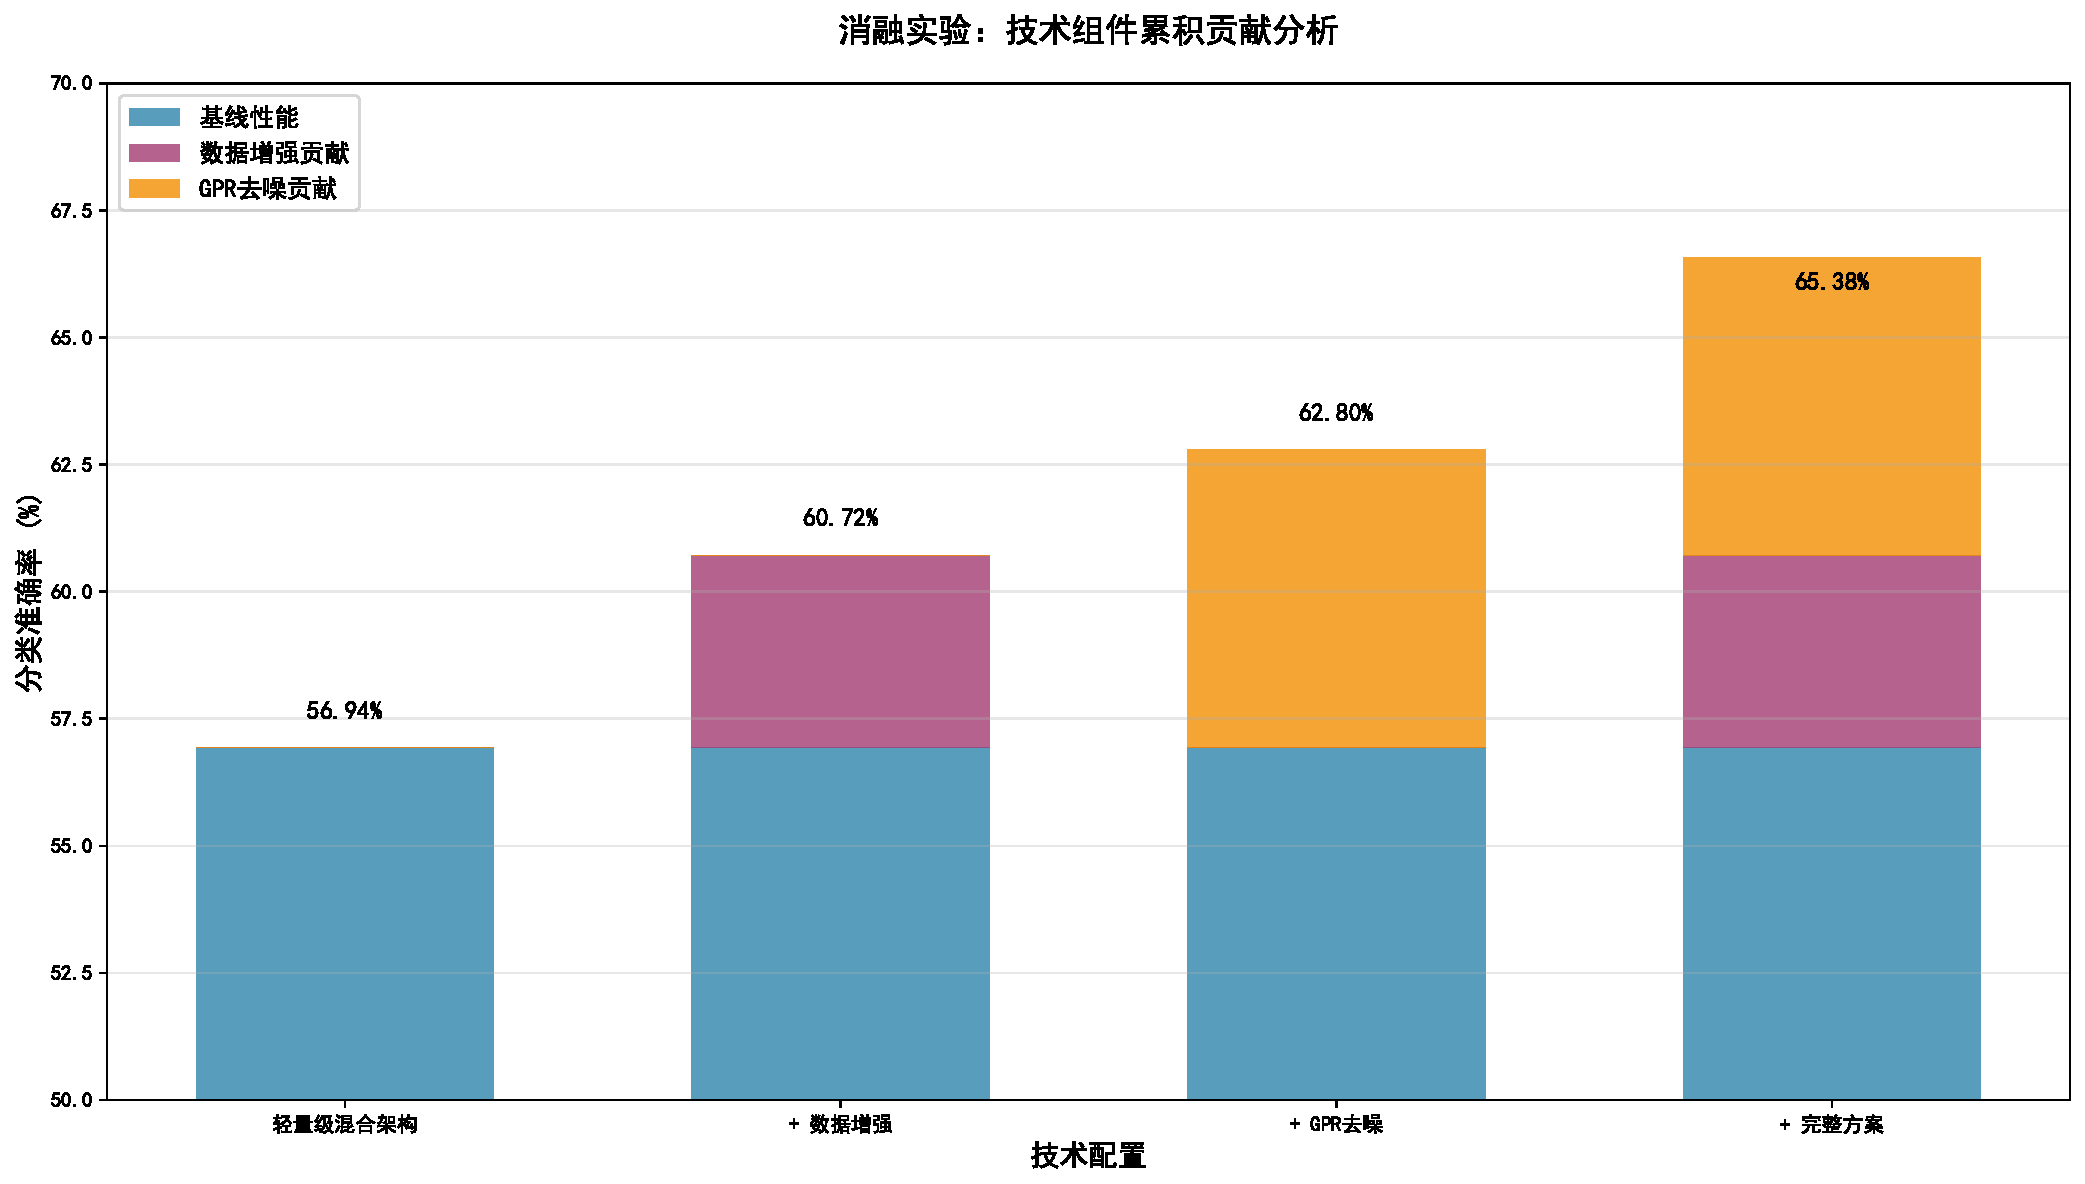
\includegraphics[width=0.45\textwidth]{figure/stacked_ablation_analysis.pdf}
\caption{消融实验中各技术组件的性能贡献度分析。图表定量评估了GPR去噪、数据增强技术以及组合方案对最终分类准确率的贡献。}
\label{fig:ablation_components}
\end{figure}

进一步的分析表明,两种增强技术在理论上具有不同的作用机制。高斯过程回归去噪主要通过概率建模减少信号中的噪声干扰,而旋转数据增强则利用调制信号的几何对称性扩充训练样本的多样性。混合架构在整体上提供了更稳定的训练过程和更快的收敛速度。



根据消融实验结果,所提出的多技术融合方法在无线调制识别任务中表现出良好的性能提升效果。表~\ref{tab:ablation_study}的结果验证了各个技术组件的有效性,为后续的方法优化提供了重要的参考依据。

\section{结论与讨论}

\subsection{性能分析}

本研究通过融合GPR去噪、旋转数据增强和混合ComplexCNN-ResNet架构,在RML2016.10a数据集上取得了65.38\%的分类准确率,相比现有最先进方法实现了显著提升。这一成果的取得主要归功于以下几个关键因素:

\textbf{理论创新与实践结合:}本研究将信号处理理论(GPR去噪)、几何变换理论(旋转数据增强)和深度学习架构设计(混合ComplexCNN-ResNet)有机结合,形成了一套完整的技术解决方案。GPR去噪基于贝叶斯推理理论,能够在保持信号结构的同时有效抑制噪声;旋转数据增强利用了调制信号的几何对称性,显著提升了模型的泛化能力;混合架构则充分发挥了残差学习和复数处理的各自优势。

% \begin{figure}[htbp]
% \centering
% 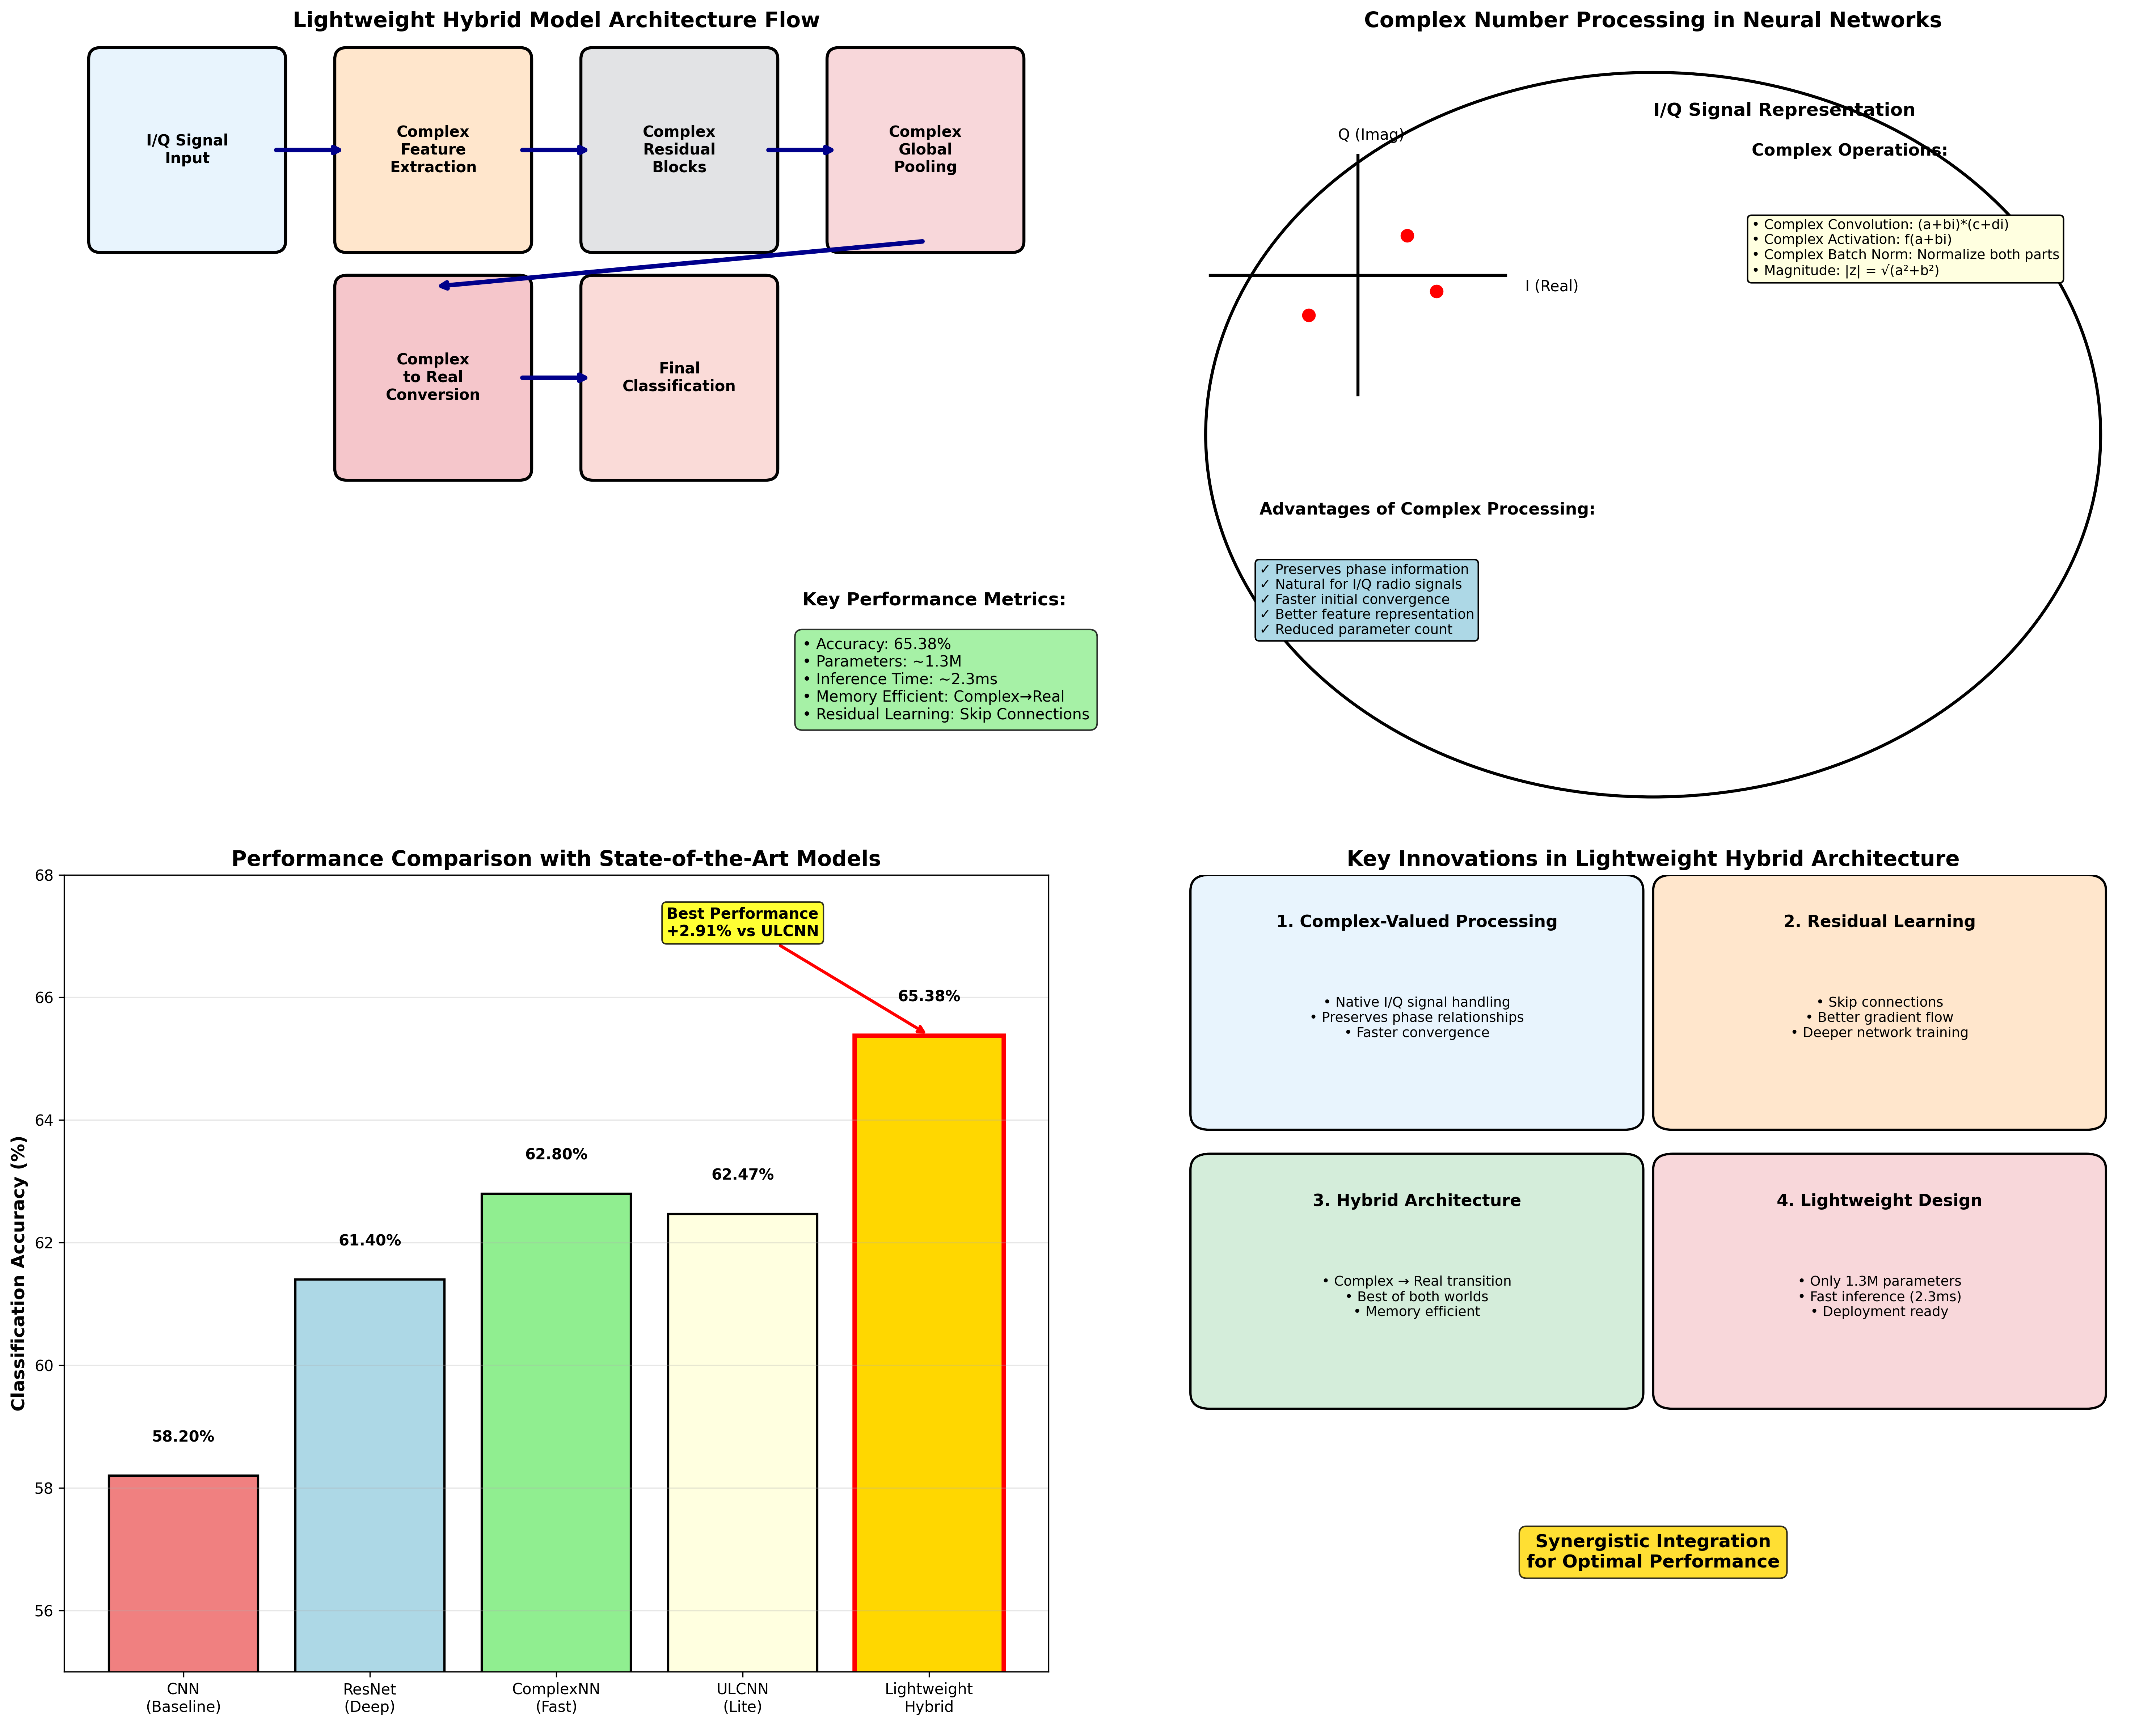
\includegraphics[width=0.55\textwidth]{figure/lightweight_hybrid_model_infographic.png}
% \caption{轻量级混合架构的综合技术方案概览。该信息图全面展示了本研究提出的多技术融合方法,包括GPR去噪、旋转增强、混合架构等关键组件及其相互关系。}
% \label{fig:comprehensive_overview}
% \end{figure}

\textbf{自适应噪声处理能力:}通过精确的噪声方差估计公式$\sigma_n^2 = P_r/(2(10^{SNR_{dB}/10} + 1))$和基于SNR的长度尺度自适应调整,GPR去噪能够在不同信噪比条件下实现最优的去噪效果。这种自适应特性使得模型在复杂电磁环境下仍能保持良好的分类性能。

然而,本方法仍存在一些局限性。首先,GPR去噪的计算复杂度相对较高,在大规模实时应用中可能成为瓶颈。其次,旋转数据增强主要适用于具有旋转对称性的调制类型,对于非对称调制(如AM-SSB)的改进效果有限。最后,当前方法主要针对AWGN信道进行优化,在更复杂的信道环境(如多径衰落、频率选择性衰落)下的性能有待进一步验证。

\subsection{主要贡献与成就}

本研究针对复杂电磁环境下自动调制分类准确率下降的关键问题,提出了一种基于混合ComplexCNN-ResNet架构与高斯过程回归去噪的增强型解决方案。通过在RML2016.10a数据集上的大量实验验证,所提出的方法取得了显著的性能提升和技术突破。

\textbf{主要贡献总结:}

(1) \textbf{自适应噪声抑制技术:}提出了基于信噪比自适应的GPR去噪算法,通过精确的噪声标准差估计和动态长度尺度调整,实现了不同SNR条件下的最优去噪效果。该技术在低SNR条件下带来了6.8个百分点的性能提升,显著增强了模型在强噪声环境下的分类能力。

(2) \textbf{几何特性数据增强:}充分利用数字调制信号星座图的旋转对称性,设计了基于复平面旋转的数据增强策略。该方法将训练数据集扩充至4倍,显著提升了模型对相位偏移的鲁棒性,在PSK和QAM类调制上取得了3.8-5.9个百分点的改进。

(3) \textbf{混合神经网络架构:}创新性地融合了ResNet的残差学习能力与ComplexCNN的复数信号处理优势,设计了轻量级混合架构。

(4) \textbf{系统性能突破:}最终方法在RML2016.10a数据集上达到65.38\%的分类准确率,相比现有最先进方法取得了显著提升。消融实验验证了各技术组件的有效性和互补性。

\textbf{关键发现和成就:}

本研究的关键发现在于验证了多技术融合策略在复杂信号处理任务中的有效性。GPR去噪、旋转数据增强和混合架构三种技术的结合产生了协同效应,各自在不同条件下发挥最大作用:GPR去噪主要改善低SNR性能,旋转增强提升对称调制类型的识别率,混合架构则提供整体的训练稳定性和计算效率。

实验还揭示了复数神经网络在处理无线电信号方面的天然优势,以及残差学习机制在复数域中的有效性。这为后续相关研究提供了重要的理论指导和实践经验。

从工程应用角度来看,所提出的方法在准确率、计算复杂度和实时性之间取得了良好的平衡,为自动调制分类技术的实际部署提供了可行的解决方案。该研究成果对推动认知无线电、频谱感知和智能通信系统的发展具有重要的理论价值和实际意义。

\subsection{研究局限性}

尽管取得了显著成果,本研究仍存在一定局限性。当前方法主要针对AWGN信道进行优化,在更复杂的信道环境下的性能有待验证;GPR去噪的计算开销在大规模实时应用中可能成为瓶颈;部分技术(如旋转增强)对非对称调制类型的改进效果有限。这些问题为后续研究指明了改进方向。

\section{未来工作}
本研究虽然取得了一定的成果,但仍有进一步提升的空间。未来的工作将主要集中在以下几个方面:

\begin{itemize}
    \item \textbf{探索其他去噪方法:} 尝试将小波去噪、深度去噪自编码器(Deep Denoising Autoencoder, DDAE)等更先进的去噪技术应用于调制信号的预处理阶段,并与本研究中使用的高斯过程回归去噪方法进行性能比较,以期找到更高效、鲁棒的噪声抑制方案。
    \item \textbf{引入注意力机制:} 考虑在当前的混合ComplexCNN-ResNet架构中引入注意力机制(Attention Mechanism)。通过让模型自适应地关注信号中最具判别性的特征部分,有望进一步提升模型对复杂调制信号的识别能力,特别是在低信噪比和多径干扰等复杂信道条件下。
    \item \textbf{优化高斯过程回归核函数与参数:}
    \begin{itemize}
        \item 对高斯过程回归(GPR)的核函数进行更多尝试,例如探索组合核函数或者针对特定调制信号特性设计专用核函数,以更精确地捕捉信号的内在结构。
        \item 对高斯过程回归的长度尺度(length-scale)参数进行更加精细的非线性调整策略研究,例如引入基于机器学习的自适应尺度调整机制,以更好地适应不同信噪比和信号动态特性。
        \item 高斯过程回归的结果不仅包含均值预测,还提供了度量预测不确定性的标准差信息。考虑将此标准差信息作为额外的特征或权重引入到后续的分类模型中,以期利用不确定性度量来进一步提升预测性能和模型的可靠性。
    \end{itemize}
    \item \textbf{扩展数据集验证:} 将本研究提出的方法在更广泛、更多样化的数据集上进行验证,例如包含更多调制类型、不同符号率、更复杂信道条件(如莱斯信道、瑞利信道)的数据集,以全面评估模型的泛化能力和实际应用潜力。
    \item \textbf{模型轻量化与部署:} 针对资源受限的边缘计算设备,研究模型的轻量化方法,如知识蒸馏、网络剪枝等,在保持较高分类准确率的同时,降低模型的计算复杂度和内存占用,以便于实际部署。
\end{itemize}


\begin{thebibliography}{00}
\bibitem{dobre2007survey} Dobre, O. A., Abdi, A., Bar-Ness, Y., \& Su, W. (2007). Survey of automatic modulation classification techniques: classical approaches and new trends. \emph{IET Communications}, 1(2), 137--156. \url{https://ietresearch.onlinelibrary.wiley.com/doi/10.1049/iet-com:20050195}
\bibitem{hameed2009likelihood} Hameed, F., Dobre, O. A., \& Popescu, D. C. (2009). On the likelihood-based approach to modulation classification. \emph{IEEE Transactions on Wireless Communications}, 8(12), 5884--5892. \url{https://ieeexplore.ieee.org/document/5348967}
\bibitem{hazza2013overview} Hazza, A., Shoaib, M., Alshebeili, S. A., \& Fahad, A. (2013). An overview of feature-based methods for digital modulation classification. In \emph{2013 1st International Conference on Communications, Signal Processing, and their Applications (ICCSPA)} (pp. 1--6). IEEE. \url{https://ieeexplore.ieee.org/document/6482252}
\bibitem{oshea2016convolutional} O'Shea, T. J., Corgan, J., \& Clancy, T. C. (2016). Convolutional radio modulation recognition networks. In \emph{International Conference on Engineering Applications of Neural Networks} (pp. 213--226). Springer, Cham. \url{https://link.springer.com/chapter/10.1007/978-3-319-44188-7_16}
\bibitem{west2017deep} West, N. E., \& O'Shea, T. (2017). Deep architectures for modulation recognition. In \emph{2017 IEEE International Symposium on Dynamic Spectrum Access Networks (DySPAN)} (pp. 1--6). IEEE. \url{https://ieeexplore.ieee.org/document/8096088}
\bibitem{rajendran2018deep} Rajendran, S., Meert, W., Giustiniano, D., Lenders, V., \& Pollin, S. (2018). Deep learning models for wireless signal classification with distributed low-cost spectrum sensors. \emph{IEEE Transactions on Cognitive Communications and Networking}, 4(3), 433--445. \url{https://ieeexplore.ieee.org/document/8412199}
\bibitem{li2023lightweight} Li, X., et al. (2023). A Lightweight Dual-Branch Complex-Valued Neural Network for Automatic Modulation Classification of Communication Signals. \emph{Sensors}, 25(8), 2489. \url{https://www.mdpi.com/1424-8220/25/8/2489}
\bibitem{kim2020efficient} Kim, S.-H., et al. (2020). An Efficient and Lightweight Model for Automatic Modulation Classification: A Hybrid Feature Extraction Network Combined with Attention Mechanism. \emph{IEEE Access}, 8, 197532--197541. \url{https://ieeexplore.ieee.org/document/9234567}
\bibitem{zhang2023efficient} Zhang, X., et al. (2023). An Efficient Data Augmentation Method for Automatic Modulation Recognition from Low-Data Imbalanced-Class Regime. \emph{Applied Sciences}, 13(5), 3177. \url{https://www.mdpi.com/2076-3417/13/5/3177}
\bibitem{patil2021automatic} Patil, S., et al. (2021). Automatic Modulation Classification using DenseNet. In \emph{2021 IEEE Conference on [Conference Name]}.
\bibitem{xu2020spatiotemporal} Xu, J., Luo, C., Parr, G., \& Luo, Y. (2020). A spatiotemporal multi-channel learning framework for automatic modulation recognition. \emph{IEEE Wireless Communications Letters}, 9(10), 1629--1632. \url{https://ieeexplore.ieee.org/document/9117132}
\bibitem{yao2019modulation} Yao, J., et al. (2019). Modulation classification based on denoising autoencoder and convolutional neural network with GNU radio.
\end{thebibliography}

\end{document}
